%% bare_conf.tex
%% V1.4b
%% 2015/08/26
%% by Michael Shell
%% See:
%% http://www.michaelshell.org/
%% for current contact information.
%%
%% This is a skeleton file demonstrating the use of IEEEtran.cls
%% (requires IEEEtran.cls version 1.8b or later) with an IEEE
%% conference paper.
%%
%% Support sites:
%% http://www.michaelshell.org/tex/ieeetran/
%% http://www.ctan.org/pkg/ieeetran
%% and
%% http://www.ieee.org/

%%*************************************************************************
%% Legal Notice:
%% This code is offered as-is without any warranty either expressed or
%% implied; without even the implied warranty of MERCHANTABILITY or
%% FITNESS FOR A PARTICULAR PURPOSE! 
%% User assumes all risk.
%% In no event shall the IEEE or any contributor to this code be liable for
%% any damages or losses, including, but not limited to, incidental,
%% consequential, or any other damages, resulting from the use or misuse
%% of any information contained here.
%%
%% All comments are the opinions of their respective authors and are not
%% necessarily endorsed by the IEEE.
%%
%% This work is distributed under the LaTeX Project Public License (LPPL)
%% ( http://www.latex-project.org/ ) version 1.3, and may be freely used,
%% distributed and modified. A copy of the LPPL, version 1.3, is included
%% in the base LaTeX documentation of all distributions of LaTeX released
%% 2003/12/01 or later.
%% Retain all contribution notices and credits.
%% ** Modified files should be clearly indicated as such, including  **
%% ** renaming them and changing author support contact information. **
%%*************************************************************************


% *** Authors should verify (and, if needed, correct) their LaTeX system  ***
% *** with the testflow diagnostic prior to trusting their LaTeX platform ***
% *** with production work. The IEEE's font choices and paper sizes can   ***
% *** trigger bugs that do not appear when using other class files.       ***                          
% The testflow support page is at:
% http://www.michaelshell.org/tex/testflow/

\documentclass[conference]{IEEEtran}
% Some Computer Society conferences also require the compsoc mode option,
% but others use the standard conference format.
%
% If IEEEtran.cls has not been installed into the LaTeX system files,
% manually specify the path to it like:
% \documentclass[conference]{../sty/IEEEtran}

\usepackage{booktabs}
\newcommand{\ra}[1]{\renewcommand{\arraystretch}{#1}}

\usepackage[usenames,dvipsnames]{color}
\newcommand{\todo}[1]
  {{\scriptsize \textbf{\color{red} {#1}}}}



% Some very useful LaTeX packages include:
% (uncomment the ones you want to load)


% *** MISC UTILITY PACKAGES ***
%
%\usepackage{ifpdf}
% Heiko Oberdiek's ifpdf.sty is very useful if you need conditional
% compilation based on whether the output is pdf or dvi.
% usage:
% \ifpdf
%   % pdf code
% \else
%   % dvi code
% \fi
% The latest version of ifpdf.sty can be obtained from:
% http://www.ctan.org/pkg/ifpdf
% Also, note that IEEEtran.cls V1.7 and later provides a builtin
% \ifCLASSINFOpdf conditional that works the same way.
% When switching from latex to pdflatex and vice-versa, the compiler may
% have to be run twice to clear warning/error messages.


\usepackage{listings}



% *** CITATION PACKAGES ***
%
\usepackage{cite}
% cite.sty was written by Donald Arseneau
% V1.6 and later of IEEEtran pre-defines the format of the cite.sty package
% \cite{} output to follow that of the IEEE. Loading the cite package will
% result in citation numbers being automatically sorted and properly
% "compressed/ranged". e.g., [1], [9], [2], [7], [5], [6] without using
% cite.sty will become [1], [2], [5]--[7], [9] using cite.sty. cite.sty's
% \cite will automatically add leading space, if needed. Use cite.sty's
% noadjust option (cite.sty V3.8 and later) if you want to turn this off
% such as if a citation ever needs to be enclosed in parenthesis.
% cite.sty is already installed on most LaTeX systems. Be sure and use
% version 5.0 (2009-03-20) and later if using hyperref.sty.
% The latest version can be obtained at:
% http://www.ctan.org/pkg/cite
% The documentation is contained in the cite.sty file itself.






% *** GRAPHICS RELATED PACKAGES ***
%
\ifCLASSINFOpdf
   \usepackage[pdftex]{graphicx}
  % declare the path(s) where your graphic files are
   \graphicspath{{images/}}
  % and their extensions so you won't have to specify these with
  % every instance of \includegraphics
   \DeclareGraphicsExtensions{.pdf,.jpeg,.png, .jpg}
\else
  % or other class option (dvipsone, dvipdf, if not using dvips). graphicx
  % will default to the driver specified in the system graphics.cfg if no
  % driver is specified.
  % \usepackage[dvips]{graphicx}
  % declare the path(s) where your graphic files are
  % \graphicspath{{../eps/}}
  % and their extensions so you won't have to specify these with
  % every instance of \includegraphics
  % \DeclareGraphicsExtensions{.eps}
\fi
% graphicx was written by David Carlisle and Sebastian Rahtz. It is
% required if you want graphics, photos, etc. graphicx.sty is already
% installed on most LaTeX systems. The latest version and documentation
% can be obtained at: 
% http://www.ctan.org/pkg/graphicx
% Another good source of documentation is "Using Imported Graphics in
% LaTeX2e" by Keith Reckdahl which can be found at:
% http://www.ctan.org/pkg/epslatex
%
% latex, and pdflatex in dvi mode, support graphics in encapsulated
% postscript (.eps) format. pdflatex in pdf mode supports graphics
% in .pdf, .jpeg, .png and .mps (metapost) formats. Users should ensure
% that all non-photo figures use a vector format (.eps, .pdf, .mps) and
% not a bitmapped formats (.jpeg, .png). The IEEE frowns on bitmapped formats
% which can result in "jaggedy"/blurry rendering of lines and letters as
% well as large increases in file sizes.
%
% You can find documentation about the pdfTeX application at:
% http://www.tug.org/applications/pdftex





% *** MATH PACKAGES ***
%
\usepackage{amsmath}
% A popular package from the American Mathematical Society that provides
% many useful and powerful commands for dealing with mathematics.
%
% Note that the amsmath package sets \interdisplaylinepenalty to 10000
% thus preventing page breaks from occurring within multiline equations. Use:
%\interdisplaylinepenalty=2500
% after loading amsmath to restore such page breaks as IEEEtran.cls normally
% does. amsmath.sty is already installed on most LaTeX systems. The latest
% version and documentation can be obtained at:
% http://www.ctan.org/pkg/amsmath





% *** SPECIALIZED LIST PACKAGES ***
%
%\usepackage{algorithmic}
% algorithmic.sty was written by Peter Williams and Rogerio Brito.
% This package provides an algorithmic environment fo describing algorithms.
% You can use the algorithmic environment in-text or within a figure
% environment to provide for a floating algorithm. Do NOT use the algorithm
% floating environment provided by algorithm.sty (by the same authors) or
% algorithm2e.sty (by Christophe Fiorio) as the IEEE does not use dedicated
% algorithm float types and packages that provide these will not provide
% correct IEEE style captions. The latest version and documentation of
% algorithmic.sty can be obtained at:
% http://www.ctan.org/pkg/algorithms
% Also of interest may be the (relatively newer and more customizable)
% algorithmicx.sty package by Szasz Janos:
% http://www.ctan.org/pkg/algorithmicx




% *** ALIGNMENT PACKAGES ***
%
%\usepackage{array}
% Frank Mittelbach's and David Carlisle's array.sty patches and improves
% the standard LaTeX2e array and tabular environments to provide better
% appearance and additional user controls. As the default LaTeX2e table
% generation code is lacking to the point of almost being broken with
% respect to the quality of the end results, all users are strongly
% advised to use an enhanced (at the very least that provided by array.sty)
% set of table tools. array.sty is already installed on most systems. The
% latest version and documentation can be obtained at:
% http://www.ctan.org/pkg/array


% IEEEtran contains the IEEEeqnarray family of commands that can be used to
% generate multiline equations as well as matrices, tables, etc., of high
% quality.




% *** SUBFIGURE PACKAGES ***
%\ifCLASSOPTIONcompsoc
%  \usepackage[caption=false,font=normalsize,labelfont=sf,textfont=sf]{subfig}
%\else
%  \usepackage[caption=false,font=footnotesize]{subfig}
%\fi
% subfig.sty, written by Steven Douglas Cochran, is the modern replacement
% for subfigure.sty, the latter of which is no longer maintained and is
% incompatible with some LaTeX packages including fixltx2e. However,
% subfig.sty requires and automatically loads Axel Sommerfeldt's caption.sty
% which will override IEEEtran.cls' handling of captions and this will result
% in non-IEEE style figure/table captions. To prevent this problem, be sure
% and invoke subfig.sty's "caption=false" package option (available since
% subfig.sty version 1.3, 2005/06/28) as this is will preserve IEEEtran.cls
% handling of captions.
% Note that the Computer Society format requires a larger sans serif font
% than the serif footnote size font used in traditional IEEE formatting
% and thus the need to invoke different subfig.sty package options depending
% on whether compsoc mode has been enabled.
%
% The latest version and documentation of subfig.sty can be obtained at:
% http://www.ctan.org/pkg/subfig




% *** FLOAT PACKAGES ***
%
%\usepackage{fixltx2e}
% fixltx2e, the successor to the earlier fix2col.sty, was written by
% Frank Mittelbach and David Carlisle. This package corrects a few problems
% in the LaTeX2e kernel, the most notable of which is that in current
% LaTeX2e releases, the ordering of single and double column floats is not
% guaranteed to be preserved. Thus, an unpatched LaTeX2e can allow a
% single column figure to be placed prior to an earlier double column
% figure.
% Be aware that LaTeX2e kernels dated 2015 and later have fixltx2e.sty's
% corrections already built into the system in which case a warning will
% be issued if an attempt is made to load fixltx2e.sty as it is no longer
% needed.
% The latest version and documentation can be found at:
% http://www.ctan.org/pkg/fixltx2e


%\usepackage{stfloats}
% stfloats.sty was written by Sigitas Tolusis. This package gives LaTeX2e
% the ability to do double column floats at the bottom of the page as well
% as the top. (e.g., "\begin{figure*}[!b]" is not normally possible in
% LaTeX2e). It also provides a command:
%\fnbelowfloat
% to enable the placement of footnotes below bottom floats (the standard
% LaTeX2e kernel puts them above bottom floats). This is an invasive package
% which rewrites many portions of the LaTeX2e float routines. It may not work
% with other packages that modify the LaTeX2e float routines. The latest
% version and documentation can be obtained at:
% http://www.ctan.org/pkg/stfloats
% Do not use the stfloats baselinefloat ability as the IEEE does not allow
% \baselineskip to stretch. Authors submitting work to the IEEE should note
% that the IEEE rarely uses double column equations and that authors should try
% to avoid such use. Do not be tempted to use the cuted.sty or midfloat.sty
% packages (also by Sigitas Tolusis) as the IEEE does not format its papers in
% such ways.
% Do not attempt to use stfloats with fixltx2e as they are incompatible.
% Instead, use Morten Hogholm'a dblfloatfix which combines the features
% of both fixltx2e and stfloats:
%
% \usepackage{dblfloatfix}
% The latest version can be found at:
% http://www.ctan.org/pkg/dblfloatfix



\usepackage{amsmath}
\usepackage{amsfonts}
\usepackage{amssymb}
\usepackage{graphicx}

% INCLUDE THIS
\usepackage{listings, lstautogobble}

% *** PDF, URL AND HYPERLINK PACKAGES ***
%
\usepackage{url}
% url.sty was written by Donald Arseneau. It provides better support for
% handling and breaking URLs. url.sty is already installed on most LaTeX
% systems. The latest version and documentation can be obtained at:
% http://www.ctan.org/pkg/url
% Basically, \url{my_url_here}.




% *** Do not adjust lengths that control margins, column widths, etc. ***
% *** Do not use packages that alter fonts (such as pslatex).         ***
% There should be no need to do such things with IEEEtran.cls V1.6 and later.
% (Unless specifically asked to do so by the journal or conference you plan
% to submit to, of course. )


% correct bad hyphenation here
\hyphenation{op-tical net-works semi-conduc-tor}

\usepackage{microtype}
\usepackage{lipsum}
\usepackage{multicol}

\usepackage{array}
\usepackage{tabulary}
\newcolumntype{K}[1]{>{\arraybackslash}p{#1}}

\usepackage{array}
\newcolumntype{C}[1]{>{\centering\arraybackslash}m{#1}}
\newcolumntype{R}[1]{>{\raggedleft\arraybackslash}m{#1}}

\usepackage{adjustbox}

 
\pagenumbering{arabic}
\begin{document}
%
% paper title
% Titles are generally capitalized except for words such as a, an, and, as,
% at, but, by, for, in, nor, of, on, or, the, to and up, which are usually
% not capitalized unless they are the first or last word of the title.
% Linebreaks  can be used within to get better formatting as desired.
% Do not put math or special symbols in the title.
\title{Using a probabilistic model to predict bug fixes}


% author names and affiliations
% use a multiple column layout for up to three different
% affiliations

\author{\IEEEauthorblockN{Authors hidden for the purposes of double blind review}
\IEEEauthorblockA{\\
\\
\\}

%REPLACE FOR CAMERA READY:
%\author{\IEEEauthorblockN{Mauricio Soto}
%\IEEEauthorblockA{Carnegie Mellon University\\
%Pittsburgh PA\\
%mauriciosoto@cmu.edu}
%\and
%\IEEEauthorblockN{Claire Le Goues}
%\IEEEauthorblockA{Carnegie Mellon University\\
%Pittsburgh PA\\
%clegoues@cs.cmu.edu}




%\and
%\IEEEauthorblockN{James Kirk\\ and Montgomery Scott}
%\IEEEauthorblockA{Starfleet Academy\\
%San Francisco, California 96678--2391\\
%Telephone: (800) 555--1212\\
%Fax: (888) 555--1212}

}

% conference papers do not typically use \thanks and this command
% is locked out in conference mode. If really needed, such as for
% the acknowledgment of grants, issue a \IEEEoverridecommandlockouts
% after \documentclass

% for over three affiliations, or if they all won't fit within the width
% of the page, use this alternative format:
% 
%\author{\IEEEauthorblockN{Michael Shell\IEEEauthorrefmark{1},
%Homer Simpson\IEEEauthorrefmark{2},
%James Kirk\IEEEauthorrefmark{3}, 
%Montgomery Scott\IEEEauthorrefmark{3} and
%Eldon Tyrell\IEEEauthorrefmark{4}}
%\IEEEauthorblockA{\IEEEauthorrefmark{1}School of Electrical and Computer Engineering\\
%Georgia Institute of Technology,
%Atlanta, Georgia 30332--0250\\ Email: see http://www.michaelshell.org/contact.html}
%\IEEEauthorblockA{\IEEEauthorrefmark{2}Twentieth Century Fox, Springfield, USA\\
%Email: homer@thesimpsons.com}
%\IEEEauthorblockA{\IEEEauthorrefmark{3}Starfleet Academy, San Francisco, California 96678-2391\\
%Telephone: (800) 555--1212, Fax: (888) 555--1212}
%\IEEEauthorblockA{\IEEEauthorrefmark{4}Tyrell Inc., 123 Replicant Street, Los Angeles, California 90210--4321}}




% use for special paper notices
%\IEEEspecialpapernotice{(Invited Paper)}




% make the title area
\maketitle

% As a general rule, do not put math, special symbols or citations
% in the abstract
\begin{abstract}
Automatic Software Repair (APR) has significant potential to reduce software
maintenance costs by reducing the human effort required to localize and fix
bugs. Well-known state-of-the-art generate-and-validate 
APR approaches select between and instantiate various mutation operators
to construct candidate patches, informed by largely heuristic probability
distributions.  This may reduce effectiveness in terms of both efficiency and
output quality; patches informed by the ways humans fix bugs may be considered
more acceptable.  In practice, human developers
have many options in terms of how to edit code to fix bugs, some of which 
are far more common than others (e.g., deleting a line of code is more common
than adding a new class).
Treating such edits as 
APR mutation operators, we  
mined the most recent 100 bug-fixing commits from each of the 500 most popular Java projects in Github (largest 
dataset to date) to
create a probabilistic model describing edit distributions.
We categorize, compare and evaluate the different mutation operators used in 
the state of the art approaches. Finally, we mine association rules to analyze context surrounding
multi-edit source code changes, an understudied problem 
that covers the majority of real source code changes. Our evaluation
indicates that by applying the probabilistic model we are able to find
the correct mutation operator to patch bugs faster in the majority of bugs
studied, and that using the superset of all mutation operators performs better than restricting the mutation operator pool to just one category.  
\end{abstract}


% no keywords




% For peer review papers, you can put extra information on the cover
% page as needed:
% \ifCLASSOPTIONpeerreview
% \begin{center} \bfseries EDICS Category: 3-BBND \end{center}
% \fi
%
% For peerreview papers, this IEEEtran command inserts a page break and
% creates the second title. It will be ignored for other modes.
\IEEEpeerreviewmaketitle



\section{Introduction} \label{introduction}
% no \IEEEPARstart
Repairing errors is one of the most expensive\cite{Tassey02,Britton13} and 
resource consuming~\cite{Weiss07} tasks in 
the software development process, especially for large error-prone systems~\cite{Liblit03,Anvik05} in modern languages that have to comply with standards of scalability and 
maintainability.

There have been efforts to automate this complex task by 
building automatic program repair tools that are able to automatically repair 
bugs in 
programs~\cite{legoues12,kim2013,Weimer13,fan15,long15,debroy10,perkins09,wei10}. 
One well-known class of repair techniques follows a 
\emph{generate-and-validate} approach, which take as input a test suite, 
including at
least one failing test case exposing
a defect, and source code to be 
modified.  These approaches then \emph{generate} a large patch candidate space 
by applying 
mutation operators to the original source code and \emph{validate} each by
running the patched  program against the test suite, seeking a candidate that
leads the program to pass all input test cases. 

One reason this is challenging is the vast search space of possible 
edits that can be applied to the different sections of the source 
code~\cite{long16}. Each such technique defines  a set of possible changes to be
applied to the source code, which we refer to as ``Mutation operators''; these 
operators enable program variations.
There is a broad diversity of such operators, such as deleting or inserting 
statements~\cite{legoues12}, applying templates~\cite{kim2013}, transformation 
schemas~\cite{fan15}, etc.~\footnote{In this study we will exclude 
from 
consideration semantic approaches since the main topic of interest is how 
candidate patches are created} 
Given a potentially-faulty location, many
generate-and-validate approaches (e.g., GenProg~\cite{legoues12}, 
Par~\cite{kim2013}, TrpAutoRepair~\cite{Qi13}, RSRepair~\cite{Qi14},
AE~\cite{Weimer13}) use probability distributions to inform the selection of 
which mutation operator
will be applied to construct candidate patches that are either random or adapted
from the results of a particular benchmarks. Most of these techniques and others 
use randomized search for patch 
generation~\cite{arcuri08,bradbury10,Qi14,Weimer13}.

In reality, human developers choose some mutation operators 
much more often than 
others (e.g., deleting a line of code is more common than adding a new class). In this paper we study and then simulate the behavior of human developers in order 
to create patches the closest way to what real developers do, which has 
being evaluated to create patches that are easier to understand by
humans~\cite{kim2013} and 
therefore it increases the maintainability of the patches. We follow a similar
intuition to Prophet~\cite{long15} which ranks candidate patches
according to their likelihood to fix the bug based on a model constructed by
human behavior. Unlike Prophet, we bring the
probabilistic model much earlier in the process, to where
patch candidates are created. We also include a more expressive superset of repair mutation
operators, beyond the transformation schemas~\cite{fan15}.  

The search space in automatic program repair, including the various mutation
operators used, has been growing in a relatively ad hoc 
manner. We mitigate this effect by categorizing and comparing a superset of
mutation operators in use in a number of 
state-of-the-art approaches, including GenProg~\cite{legoues12}, RSRepair~\cite{Qi14}, AE~\cite{Weimer13}, PAR~\cite{kim2013}, 
SPR~\cite{fan15},
Prophet~\cite{Long2016}, etc.
We then mine
the 500 most popular Github Java projects to produce a model of the probability of
each of the possible mutation operators used in prior approaches based on 
empirical data that describes how human programmers fix their code.  We use this
model to inform a repair approach that chooses from the set of possible
operators based on 
probabilities that describe how often each is used
to fix bugs in real world projects. 

We evaluate this approach both on its own, by evaluating the predictive power of
the model by analyzing the number of correctly predicted mutation
operators,
and as part of a repair algorithm, by applying the model to predict independent
instances. We demonstrate this algorithm with a subset of included operators in
a case study setting.  We then evaluate an APR tool with the full set of mutation
operators to compare the relative utility of our probabilistic model as compared
to a uniform model.  We perform this latter evaluation on a subset of defects
from Defects4j,~\cite{just14} a 
database and framework of reproducible real-life bugs found in large scale open 
source projects. In this final step we evaluate our model with bugs that require 
one line to be modified to patch them. 

Finally, we introduce a new approach for modeling multi-edit repairs based on
mining previous rules from historical edit data. Most of the
successful repairs from current approaches are
single-edit~\cite{Weimer13,Qi15,kim2013}.\todo{there's another reference
  here...maybe something from Arcuri and Briand circa 2011 that analyzed
  success?  Other papers reference it...check the Angelix paper, I think it
  probably cites it somewhere. RESPONSE: Are you talking about this paper?: Adaptive random testing: an illusion of effectiveness? Arcuri and Briand ISSTA'11}  Patches
consisting of several mutations have been understudied even when the vast majority
of patches in existence are multi-edit changes~\cite{Soto15}.\todo{easy reference here, maybe?
   Something from the MSR community?  Someone must have studied this. RESPONSE: We did :)}  We
 propose and initially validated an approach that predicts from a given 
single-edit mutation which operation should be applied
next to create multi-edit patches. 


The primary contributions of this paper thus are:
\begin{itemize}
  \item \textbf{New Repair Approach that generates patches based on human behavior:} that incorporates mutation operators
    from multiple state-of-the-art approaches and 
    uses a probabilistic model to between them, favoring those more commonly
    used by human developers. It is, to the best of our
    knowledge, the first study that, compares and contrasts directly using the
    same platform, all the different mutation operators from the most well known
    state of the art approaches.  \todo{Do we actually compare/draw conclusions
      on this?  We should, if we claim it.  This is mostly a note to myself to
      ensure we do.} 
    \item \textbf{Large, mined model of single-edit repairs to Java code.} To
      enable the above approach, we mine a probabilistic model for edits to Java programs
    from bug fixes to the 500 most popular projects from
    Github.   A deeper
    understanding of which mutation operators are used by programmers to fix
    errors in source code, and the frequency of each of the mutation operators
    analyzed. 
  \item \textbf{Evidence:} Evaluation of the probabilistic model in several
    different benchmarks, including a large number of real life bugs from well
    known open source projects. We conclude that by creating candidate patches using human behavior we are able to find patches faster and we found that the patch creation process benefits from combining the mutation operator categories, instead of isolating the mutation operator pool to a single category. 
  \item \textbf{Multi-edit repair approach} A proposed technique to construct 
    bug-fixing patches requiring several mutations by mining and then applying association
    rules from a large set of historical bug fixes. 
\end{itemize}

The rest of this paper proceeds as follows:
The following section entails the state of the art, general terminology and
background knowledge for automatic program repair, in particular
generation-and-validation. Section~\ref{categorization} discusses how we
categorize and generalize the mutation operators used in state of the art
approaches in an effort to compare them. Section~\ref{buildingTheModel}
describes the process of how we gathered, analyzed and extracted the data
necessary to build the probabilistic model. Section~\ref{multEdit} is a
pioneering work that discusses a new methodology to handle defects that require
various edits to patch the code. Section~\ref{evaluation} outlines our
evaluation methodology and our benchmarks.  Finally, we have a section for
Discussion (Section~\ref{discussion}), Related Work (Section~\ref{relatedWork}), and Conclusion (Section~\ref{conclusion}).

\section{Generate-and-validate repair} \label{background}

One of the most well known approaches for automatic program repair is the
generate-and-validate approach~\cite{legoues12} which is detailed in Figure~\ref{fig:generateandvalidate}. This approach starts with source code that
has one or various bugs to be fixed, and a test suite which contains passing
test cases to guide the expected behavior of the program of the program, and failing test 
cases which expose the behavior of the program that is expected but the output
of the expected behavior does not match the output of the source code as is.



\begin{figure}[!h]
  \centering
    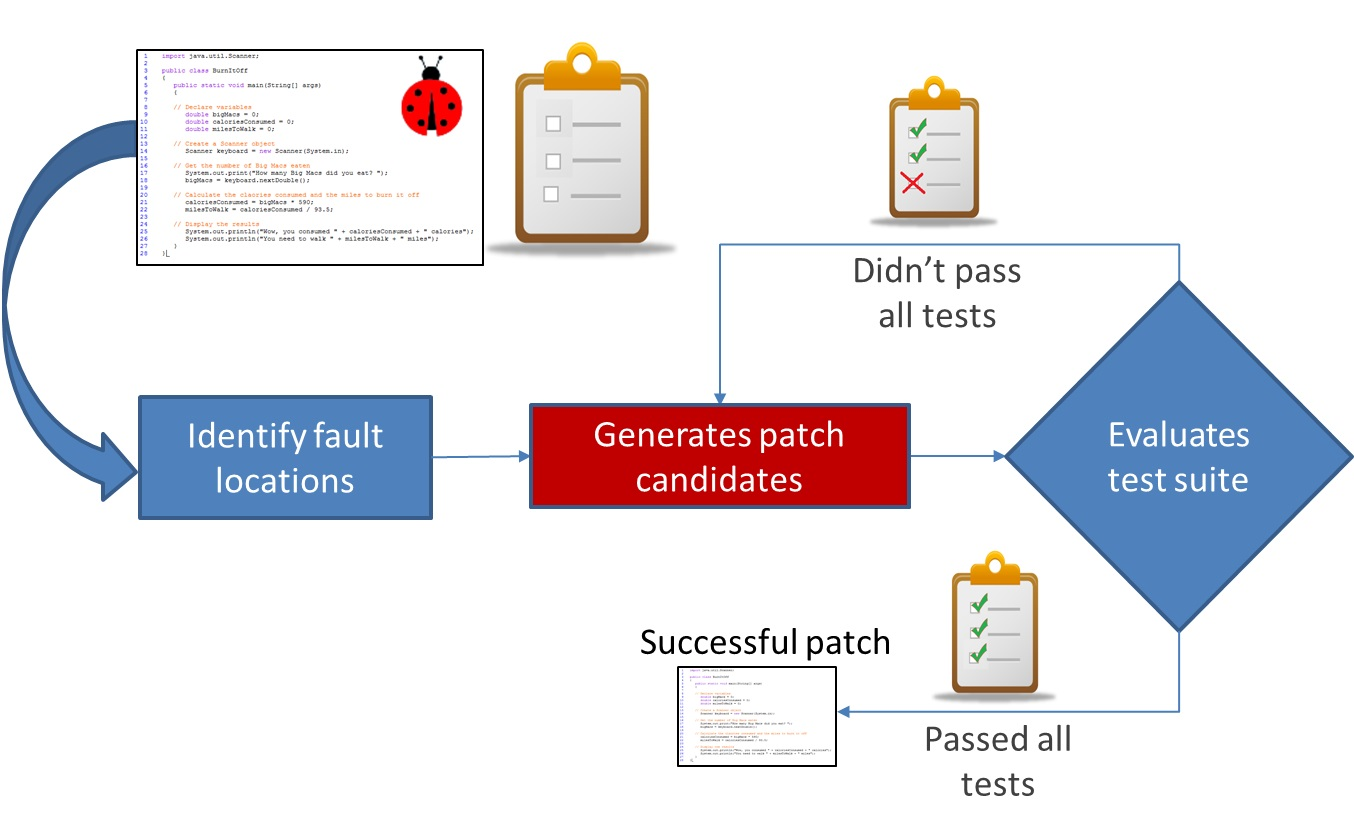
\includegraphics[scale=0.25]{Picture1}
  \caption{Generate and validate approach}
  \label{fig:generateandvalidate}
\end{figure}

\subsection{Background}
The first step of this process is to localize the error in a particular 
statement. There is an extensive set of possible approaches in literature in 
order to perform this tasks~\cite{Jones05,Jones02,Chen02,legoues12,Qi13}, also there are several papers that have focused on the evaluation of the test suite~\cite{Qi13,fan15}; the main focus of this paper will be the step between these two, as highlighted in Figure~\ref{fig:generateandvalidate} our main focus will be Generating patch candidates.

Once we know where the fault is located we proceed to create what we call 
``Candidate patches". Candidate patches are variations of the original program 
which may or may not be a patch for the bug(s) we are trying to fix. To 
create candidate patches we analyze which mutation operators can
be applied to that specific location; or if the context of that location doesn't
allow some mutation operators to be used. We apply them and once this process is finalized, as a result, there is a set of possible 
mutation operators that
can be applied to the chosen location.

Once the tool has a set of candidate patches, it will run the test suite on each 
of those candidate patches. If it is able to find a candidate patch that can 
pass all the test cases in the test suite, that candidate patch will be 
considered a patch of the bug. If it is not able to pass all the test cases in 
the test suite, then it will go back to creating more candidate patches and will 
continue to do so until it reaches a stopping point, which may be a certain user 
defined number of generations or a user defined clock time limit.

In contrast to generate-and-validate there exist other techniques used for 
automatic program repair such as Synthesis-Based program 
repair~\cite{jin11,pei14} which uses constraints to build 
correct-by-construction patches via formal verification, inferred or 
programmer-provided contracts,
or specifications~\cite{jin11,wei10}. Also in contrast to search based approaches, there exist semantic based approaches such as SemFix~\cite{nguyen13}, DirectFix~\cite{mechtaev15} and SearchRepair~\cite{ke15} which use semantic analysis to create patches for buggy code.

Regarding generate-and-validate~\cite{legoues12}, in
order to select which mutation operator will be used, the 
first step is to define in what section of the code the fault is located. This can be determined in various ways, and 
there is 
a whole set of
possible approaches that can analyze this segment with different levels of certainty and 
requiring different characteristics from the source code and/or test 
suite~\cite{Jones05,Jones02,Chen02,legoues12,Qi13,Qi2013,Abreu07,wong09}. 

\subsection{Generalization and Categorization of mutation operators} 
\label{categorization}

There are several possible mutation operators that can be applied to a location 
to modify the behavior of a program. To analyze the broad 
spectrum of mutation operators we categorized them into two groups: 
Statement-Edit and Template-Based. 

\textbf{Statement-Edit mutations:}
There is a family of well-known approaches such as GenProg~\cite{legoues12}, 
TrpAutoRepair\cite{Qi13}, RSRepair~\cite{Qi14}, and AE~\cite{Weimer13} in which the main technique for 
creating candidate 
patches is by applying coarse grained mutation operators (such as append, delete, or 
replace) which modify statements of source code to 
repair programs. A statement is  a grammar nonterminal, which in Java this translates to the smallest standalone element that expresses 
some action to be carried out, such as a while loop with its corresponding body, or a method call. These tools are able to 
apply these mutation operators to statements in the source code to 
create candidate patches.

\textbf{Template-based mutations:}
Template-based mutation operators is the family of approaches that have 
predetermined templates to apply to specific sections of the code to 
modify the behavior of the program to make it possibly fix the error in the 
code being analyzed. In this family we have well known techniques such as PAR~\cite{kim2013}, 
SPR~\cite{fan15}, and 
Prophet~\cite{Long2016}.
 
PAR is the product of a study in which researchers examined a large number of 
human 
created patches and abstracted 10 different templates to be the most 
commonly used changes that human programmers perform to fix their 
code~\cite{kim2013}.
The 10 templates which they considered in their approach are the ones detailed in Table~\ref{approachTemplates} Top.

\begin{table}[ht]
  \centering

\begin{tabular}{K{3.1cm}K{5cm}}
\hline 
\multicolumn{2}{C{8cm}}{PAR fix templates} \newline \\
\hline 
1) Null Checker & 6) Parameter Adder and Remover \\ 
2) Parameter Replacer & 7) Expression Adder and Remover \\  
3) Method Replacer & 8) Collection Size Checker \\
4) Expression Replacer & 9) Range Checker\\
5) Object Initializer & 10) Class Cast Checker\\
\end{tabular}\newline \\

\begin{tabular}{K{3.1cm}K{5cm}}
\hline 
\multicolumn{2}{C{8cm}}{PAR extra templates} \newline \\
\hline 
1) Caster Mutator & 4) Lower Bound Setter  \\
2) Castee Mutator & 5) Upper Bound Setter  \\
3) Sequence Exchanger & 6) Off-by-one Mutator\\
\end{tabular}\newline \\

\begin{tabular}{K{3.1cm}K{5cm}}
\hline 
\multicolumn{2}{C{8cm}}{SPR transformation schemas} \newline \\
\hline 
1) Condition Refinement & 4) Insert Initialization \\
2) Copy and Replace & 5) Condition Control Flow Introduction  \\
3) Value Replacement  & 6) Condition Introduction \\
\\
\end{tabular}
  \caption{(Top) PAR fix templates. (Middle) PAR extra templates. (Bottom) SPR transformation schemas.}
  \label{approachTemplates}
\end{table}

In the interest of completeness, we also include six extra templates 
mentioned on the website associated with the Par
approach.\footnote{\url{https://sites.google.com/site/autofixhkust/home/fix-templates}} 
These extra templates provide new mutation operators that helps us compare and
generalize to the other approaches; they are shown in the middle segment of
Table~\ref{approachTemplates}. 
The SPR and Prophet approaches make use of a set of transformation schemas,
shown in the Bottom section of Table~\ref{approachTemplates}.

Some of the SPR/Prophet transformation schema can be seen as a generalization of certain PAR 
templates. For example, ``\emph{Condition Introduction}'' can be seen as a superset of 
\emph{Range Checker}, \emph{Collection Size 
Checker}, \emph{Class Cast Checker}, and \emph{Null Checker}. ``\emph{Condition Refinement}" includes \emph{Expression Adder and Remover}. ``\emph{Insert Initialization}" can be 
generalized from \emph{Object Initializer}, \emph{Upper Bound Setter} and \emph{Lower Bound Setter}; ``\emph{Conditional Control Flow Introduction}" can be 
seen as a subset of \emph{Sequence Exchanger};
``\emph{Value Replacement}" can be seen as a superset of \emph{Method 
Replacer}, \emph{Parameter Replacer}, \emph{Castee Mutator} and \emph{Expression Changer}; and ``\emph{Copy 
and Replace}" can be matched to \emph{Expression Adder}. 

We also considered the program modification tool Kali~\cite{Qi15}, whose
templates can be seen as subsets of some of the PAR templates or the extensions
of the PAR templates mentioned above, for example \emph{Redirect Branch} can be seen as
a subset of ``\emph{Expression Changer}", and \emph{Insert Return and Remove Statement} are
subsets of ``\emph{Expression Adder and Remover}" accordingly. In the same way, we find
similar mutation operators that can be seen as subsets of the extensions of the
Par templates in studies such as~\cite{Offutt96,Offutt06}. 

There is enough similarity between these approaches that they can be grouped 
into one category. We have chosen the PAR templates to represent this category 
since these templates provide a more concrete description of how the code is 
being changed, in order for us to replicate it; also, as mentioned before, all the SPR, Prophet and Kali templates are represented by one or several of the PAR templates, but not viceversa; and also the PAR templates represent templates specifically for the Java language, which is a common ground for the rest of the 
approaches considered and the benchmarks to evaluate the approach on. It is also worth mentioning hybrid approaches such as HDRepair~\cite{xuan16} where the authors use a combination of previously mentioned Statement-Edit and Template-Based mutation operators.


\todo{Somewhere in this subsection we should acknowledge the techniques we don't
  consider.  The ommission of HDRepair is a notable, since it targets Java, and
  I don't think you've even cited it yet so far.  Add a reference to various
  places you mention GandV repair, at minimum, but consider adding a discussion
  of it to this framework.  Does it fit anywhere?  How?  Why/why not? RESPONSE: Do you mean to add a discussion about the semantic approaches and why we don't consider them? I added a footnote in page one regarding we not looking at semantic approaches because the main point of the paper is the way in which candidate patches are created, which, in semantic approaches is done in a completely different way.}


\section{Building the model} \label{buildingTheModel}

In this section we describe how we mined a probabilistic
model of human bug-fixing edits from a large set of popular Java projects on GitHub. 

\subsection{Selecting the corpus}

We cloned the 500 Java projects in Github 
with the most stars (as of August 2016). The methodology of 
gathering large,
popular, and active open source Java software repositories is common in
empirical studies (e.g.,~\cite{Ray14}). 
%
We compiled the most recent 100 bug fixing commits per each project. Identifying
bug fixing commits is a difficult
problem in repository mining~\cite{Bird09}. We filter these by applying a
regular expression to the commit message in each of the commits in each of the
projects that looks for words such as "fix", "bug", "issue", "problem",
etc. following the guidelines by \cite{schroter06,Cubranic05,Fischer03}. 

%\\
%\\
%$[Ff]ix(ed|es|ing)?(\backslash s)*([Bb]ug|[Ii]ssue|[Pp]roblem)?(s)?$
%\\
%\\
We also added two extra filters to our search: First we had commits that only 
modify Fava source code.  Additionally, we restrict our search to commits 
that modify a maximum of 3 files. We do this to
filter big merges of code such as pull requests or initial commits, and because
large commits are more likely to include changes unrelated to a bug fix~\cite{Dias15,Herzig13,Matsuda15,Kawrykow11}.

\subsection{Identifying mutations in developer commits}

For each bug fixing commit, we refer to the code before the fix as the
``before-fix" version and the code after as the ``after-fix" version.
We next seek to identify the changes performed between the before-fix and
after-fix versions, to analyze how often they match the mutation operators in
question. 
%
To do this we used two existing tools for mapping changes 
between two versions of code: Gumtree~\cite{falleri14}, a source code tree
differencing framework, and QACrashFix~\cite{gao15}, the tool for generating
fixes via analyzing Q\&A pages.  Specifically, we adapt QACrashFix's
differencing engine, which modifies Gumtree to account for replacements.
These tools create an AST representation of the program files for both the 
before-fix and after-fix representations of the programs for each of the files 
of the commit, and then use a set of heuristics to match the before-fix version 
with the after-fix version and produce a set of 
changes performed between them. 

For each bug-fixing commit, we greedily attempt match the identified changes to the
available 
mutation operators. For example, to identify
a Null Checker application, we go through all the actions performed to go from the
before-fix to the after-fix versions; in each of the actions we ask if the node
being manipulated is an \emph{IfStatement}, we then  ask if the action being performed
is an Insertion of a node. After we know that it is an insertion of an \emph{IfStatement}, we then ask if the first condition within the \emph{IfStatement} is an
\emph{InfixExpression} comparing an 

%  An \emph{InfixExpression} as defined by the Eclipse JDT API
% specification has the following form: 
% \\
% \\
% $InfixExpression: \\
% Expression~InfixOperator~Expression
% $
% \\
% \\  
\emph{Expression} to a
\emph{NullLiteral}. If all these conditions are met, we know that a null checker
template was applied to the code, so we count it as an instance of this template. 




%\begin{figure}[!]
%\begin{verbatim}
%var res = 0
%for (ac <- actions) {
%  if(nodeClassName(ac.getNode) 
%    == "IfStatement"){
%      if (actionName(ac) == "Insert"){
%        if((nodeClassName(ac
%          .getNode.getChildren.get(0)) 
%            == "InfixExpression") && 
%              (nodeClassName(ac
%                .getNode.getChildren
%                  .get(0).getChildren.get(1)) 
%                    == "NullLiteral")){
%                      res += 1
%      }
%    }
%  }
%}
%\end{verbatim}
%\caption{Example of heuristic to spot the template Add Null Checker}\label{fig:codeSnippet}
%\end{figure}



\subsection{Two-level probabilistic model}

\begin{figure}[!h]
  \centering
    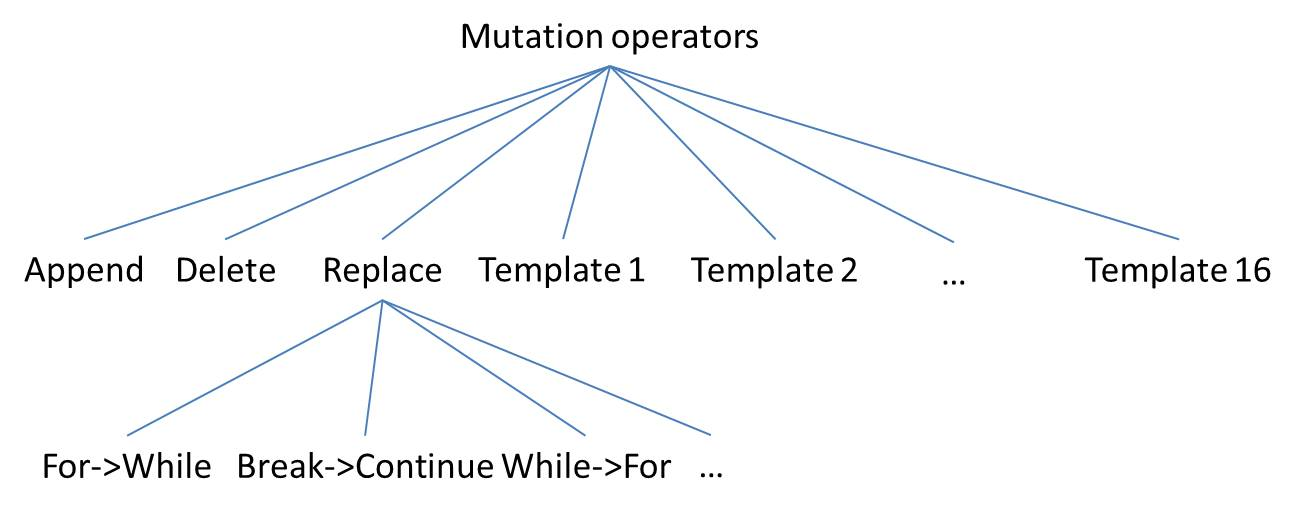
\includegraphics[scale=0.4]{Picture2}
  \caption{Two level probabilistic model}
  \label{fig:probModel}
\end{figure}

We extend an open-source implementation of the GenProg technique adapted for Java
by implementing the mutation operators from
Section~\ref{categorization} to allow the tool 
selects between the mutation operators according to the probabilities described by
a given model.\footnote{We will release a link to our implementation to support
  a camera ready; we obscure it in the interest of supporting double-blind
  review.}  We construct this model by counting incidences of all considered
mutation operators (this can be considered a generalization of a simpler
previously-proposed replacement-only model~\cite{Soto15}). The resulting model
is two-level: 

\textbf{Mutation operator probabilistic model:}
The \textit{Mutation operator probabilistic model} 
describes the probabilities of choosing between the several different mutation 
operators at a particular fault location.
%
To build the \textit{Mutation operator probabilistic model} we created 
a program that goes through these 
changes and matches these changes with the mutation operators we described 
earlier.

We sum the instances of each of the appearances of the mutation operators in the 
lists of changes created out of the differences between the before-fix and 
after-fix versions of each of the files in the 100 last bug fixing commits per 
each of the 500 projects; and these instance sums are the data we take to create 
our probabilistic model.

\textbf{Replacements probabilistic model:}
The \textit{Replacements probabilistic model}
if the ``Replacement" mutation operator is 
selected, this model describes the probability of replacing one statement with
another and thus informs the selection of fix code for such operators.
The \textit{Replacements probabilistic model} is built analogously to the
mutation operator model, 
%\footnote{https://goo.gl/mMFbnQ
but simply identifies replacements (referring to the 
``replacee" and ``replacer" statements accordingly).
%
We consider 
the 22 different types detailed by the Eclipse JDT\footnote{https://goo.gl/SX3wnA \label{stmtNames}} as
direct known subclasses of the class ``Statement", and the incidence with which
each of  
them replaces another. For example: What is the observed probability that a \texttt{For} loop 
replaces a \texttt{While} loop? Given 22 statement types, any of which may replace one
another, there are 484 possible replacement combinations. 
Note that the observed probabilities are not reciprocal, meaning 
that the probability of a \texttt{For} loop replacing a \texttt{While} loop is different from the 
probability of a \texttt{While} loop replacing a \texttt{For} loop, and the same applies to all 
the different statement types.

\subsection{Multiple edit association rule mining} 
\label{multEdit}

Single-mutation (or single-edit) source code changes are historically the most 
common subject of analysis in 
state of the art bug-fixing
approaches. This applies to both, approaches that limit the number of source 
code changes they apply to create a program variant to one change per variant 
only (eg, TrpAutoRepair~\cite{Qi13}, AE~\cite{Weimer13}, Kali~\cite{Qi15}), and 
to approaches whose search space traversal technique can allow multi-edit 
changes (eg. GenProg~\cite{legoues12}, Par~\cite{kim2013}, SPR~\cite{fan15},
Prophet~\cite{Long2016}, etc.) but typically find patches that reduce to single-edit changes.

\todo{Don't cite GenProg, Par, or HDRepair on this.You do need to say something 
like ``even  techniques that can allow multi-edit changes (like GenProg) typically find
  patches that reduce to single-edit changes.''  In fact, add that sentence
  here, with appropriate references.   I also don't think you're
  citing the correct Qi15 or Qi13 here. RESPONSE: Qi15 is Kali and Qi13 is 
TRPAutoRepair, Qi14 is RSRepair }
Although such single-edit patches can be
sufficient to repair non-trivial bugs in real software, many bug fixes in real
software require multiple edits~\cite{Weimer13}. The combination of possible mutation operators to apply in a sequence increases exponentially as we add more source code changes and the need of a mechanism to navigate this vast search space is a must when we talk about multi-edit changes.

As a first step towards mitigating this limitation, we propose 
an initial analysis of multi-edit 
source code changes by mining a more expressive model of common changes. In
particular, we are extracting \emph{association rules} between single edit changes 
to model chains of single edit changes, capturing the way humans create them.
Association rules are if/then statements that show relationships between elements in a dataset which happen frequently together.

We use the 
well known association rule mining algorithm
Apriori~\cite{Agrawal94,Liu98,Zaki2000}, which identifies frequent 
individual items in sets of transactions (commits, in our context).  We extend these sets into 
larger sets as long as those item sets appear sufficiently often in the database 
of transactions, which in our case would be the database of transactions created 
by each of the commits studied. We have divided our association rule mining to
be built one from each of the models as described in Section~\ref{armRes}. 

To extract association rules from the data gathered in our study, we 
have transformed each of the mutation operator count and replacement count from 
each of the commits studied and created a transaction to be analyzed. A transaction in this context is a row of values that describes which mutation operators were applied in a single commit.

To use Apriori we need to further clarify basic concepts used by this approach: Confidence and Support.

Formally, we define Confidence as:

\begin{center}
$conf(X \implies Y) = \dfrac{supp(X \cup Y)}{supp(X)}$ 
\end{center}

Where X and Y are possible items in a transaction. In this context it is refering to mutation operators. As seen above Confidence is calculated according to its Support, where Support is an indication of how frequently the set of mutation operators (itemset) occurs in the transaction base.
Formally, we define Support as:

\begin{center}
$supp(X) = \dfrac{|\{t \in T; X \subseteq t\}|}{|T|}$
\end{center}

Where X is the itemset being analyzed and t is each individual transaction in the database of transactions T. 

\section{Evaluation} \label{evaluation}

We evaluate our model both independently and as part of an automatic repair
technique.  We first evaluate the predictive power of the model by analyzing the
number of correctly predicted mutation operators across a large dataset, using 10 fold cross
validation to mitigate and assess the risk of overfitting
(Section~\ref{sec:generalize}).  Next, we describe a case study 
repair problem to precisely validate the increase in efficiency the
probabilistic model affords (Section~\ref{sec:casestudy}).  Finally, we evaluate
repair efficacy on fifteen real bugs from the Defects4J dataset
(Section~\ref{sec:single}), and use Apriori to create a list of the most common association rules between mutation operators mined from our corpus of the 500 more popular java projects in Github.  

To perform our evalutation, we ran our approach in a physical server that 
consists of 16 processors Intel(R) Xeon(R) CPU E5-2699 v3, with 2.30 GHz each
processor, 46080 KB cache each, and 32 GB RAM memory, operating system Ubuntu 
14.04.5 LTS.

\todo{This roadmap is imcomplete.  Add poitners to
  the multi-edit section, discussion/threats, and example patch(es), in the
  appropriate order. RESPONSE: Will add example patch soon, and modify this section accordingly.}


\subsection{Model generalization}
\label{sec:generalize}

\todo{Wait, why don't we assess the mutations model?  That seems like a natural
  experiment to have done...6 months ago, and I remember asking for it.  And
  it's the same infrastructure. RESPONSE: Because when this experiment was done the mutations model didn't exist. This first experiment on the replacements model was to know if it was worth it to make the mutations model.}
  
In this first experiment we want to evaluate the predictive power of our replacements model by analyzing once we have the faulty statement, what are the first N guesses the replacement model makes, and evaluate to what extent those first N guesses correctly predict future instances of faulty statements that need to be replaced by another statement to fix the code. We want to know if by applying the probabilistic model we will find the correct statement kind to replace it for in a larger number of instances, than using the equally distributed model. For this we will be using the percentage of instances correctly predicted when performing 10 fold cross validation~\cite{kohavi95}.

We segregated the projects that form our corpus into 10 
different folds assigned at random. For each of the 
folds we would take 1 fold for testing and the remaining 9 folds for training. 
Afterwards we analyze how often do the training data is able to predict the 
testing data. This is performed 10 times, one time per each fold and then it is 
averaged to see how commonly is the training data able to predict the testing 
data.

For each of the folds, we compare two distributions: the distribution of that fold, being used as testing 
data, and the distribution of the sub-model built from the remaining 9 folds. We want to know how many instances from the testing data are being correctly predicted by the first guesses of the training sub-model.   
  
Our overall goal is to analyze if the probabilistic model will assign a higher probability to the correct statement kind to be picked as opposed 
to the current equally distributed scheme; we rank the first five choices each 
of the models would take and see how many of the instances in the testing data 
match those first five guesses. Five guesses is the point of inflection where
the maximum difference between the two approaches happen. After five guesses, the behavior of the two models starts to become more similar to each other, until they become the same with all the twenty two possible guesses.
This is the reason why we picked five guesses as our
comparison point.

\lstdefinestyle{base}{
  language=Java,
  emptylines=1,
  breaklines=true,
  basicstyle=\ttfamily\color{black},
  moredelim=**[is][\color{red}]{@}{@},
  xleftmargin=20pt, frame=bt, basicstyle={\small\tt}, numbers=left, keywordstyle=\bfseries, 
	numberstyle=\scriptsize\tt,  moredelim=[is][\color{red}]{@}{@}, deletekeywords={}, captionpos=b, belowskip=1pt, autogobble=true
}

To illustrate the point, consider a simple example. Assume we have a 
faulty location in line 4 of the following program in our corpus:

\begin{lstlisting}[frame=single,style=base]
    List l = new LinkedList();
    int i = 0; 
    ...    
    return l.get(i); @//faulty location@
    ...
\end{lstlisting}

Assume the mutation operator model has chosen a "replace" as the mutation operator to be applied at that location. If the operator is a replacement, the next step is for the replacement model to predict what statement kind should the return be replaced by.

Since this is an instance in our corpus of bug fixes, we already know what changes the developer performed to fix it. Assume the developer performed the following change:

\begin{lstlisting}[frame=single,style=base]
    List l = new LinkedList();
    int i = 0; 
    ...    
    if(i > l.size()){
      return l.get(i);
    }    
    ...
\end{lstlisting}

What we want to know is if given a \emph{ReturnStatement} as a faulty location, would the models be able to predict that it was replaced by an \emph{IfStatement} in the first guesses. If they predict to replace it by an \emph{IfStatement} if their first guesses, then it is correctly predicted. If they do not guess it was an \emph{IfStatement} in their first five guesses, then it was not correctly predicted. We do this for all the instances distributed randomly through the different folds. 

We have a lot of these instances in the 10 folds. For example, when analyzing fold 1, we have a distribution in that fold that describes how many times each statement is replaced 
by other kinds of statements in this fold 
only. This is what we denominate testing data of this fold and we represent it with $E_{n,m}$ 
where $n$ is the statement being replaced (replacee) and $m$ the statement it is 
replaced by (replacer). Likewise, we have a probabilistic sub-model created from 
folds 2-10 inclusive $TP_{n,m}$ where $\forall n,m: 1<=n<=22 \land 1<=m<=22$, 
that describes how often each statement is replaced by 
other kinds of statements. This is what we call the training data of this fold. 



\begin{table}[ht]
\begin{tabular}{llllllllllllllllllllll}
\hline
As & Bl & Br & Cl & Co & Do & Em & EF & Ex & Fo & If \\
0\%&2\%&0\%&2\%&5\%&0\%&0\%&0\%&43\%&0\%&22\% \\
\hline 
La & Re & SC & Ca & Sw & Sy & Th & Tr & TD & VD & Wh \\
0\%&0\%&2\%&2\%&0\%&0\%&3\%&2\%&0\%&19\%&0\% \\
\hline
\end{tabular}
\\
\caption{Example of the Return Statement row of a sub-model created from 
the training data. Replacee probabillities of the replacer ReturnStatement. The acronyms represent the statement kinds detailed in footnote \ref{stmtNames}}
 \label{fig:exPredReturn} 
\end{table} 

%\begin{figure}[!h]
%  \centering
%    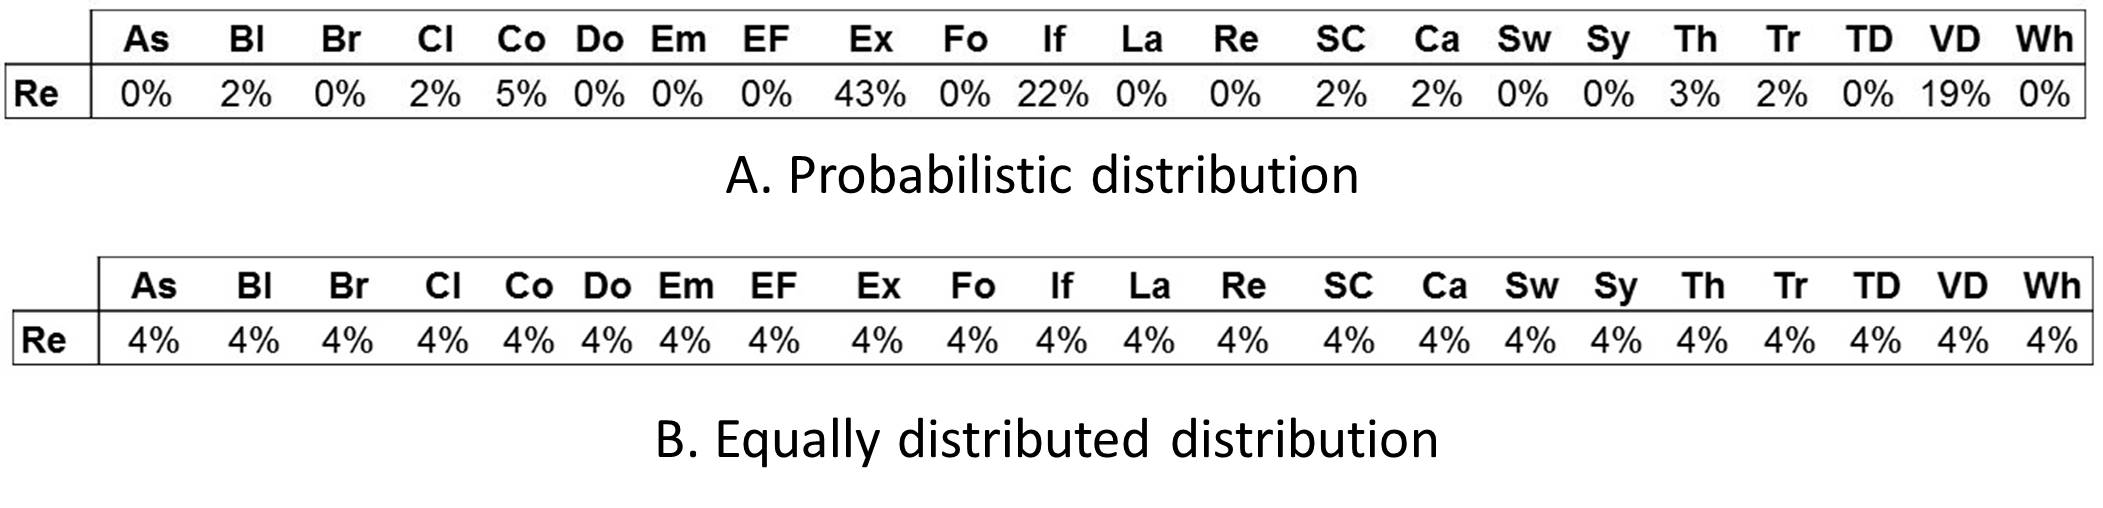
\includegraphics[scale=0.25]{sanity5}
%  \caption{A)  B) Example of return statement with equally distributed 
%probability. }
% 
%\end{figure}


In 
particular, assume we are analyzing the Return statement (Row 13). We want to 
predict 
how well the sub-model created from folds 2-10 is able to predict the testing 
data; in this particular case, how well is the section of the sub-model that 
describes the Return Statement able to predict the instance count of the 
statements that replace a Return Statement in the testing data.

Assume the training data is a sub-model $TP_{n,m}$ which contains a row 
$TP_{13,m}$ as the one shown in Figure~\ref{fig:exPredReturn}A, and the testing data is a distribution that describes 
how many instances of returns were replaced by different statements.
%as follows: 
%A return statement was replaced by a Expression Statement 4 times $E_{13,9} = 
%4$; by an If 
%Statement 2 times $E_{13,11} = 2$; by a Continue Statement 2 times $E_{13,5} = 
%2$; by a Do Statement 1 time $E_{13,6} = 1$;
%and by a Try Statement 1 time $E_{13,19} = 1$. As a clarification, this is a 
%fictional example 
%to explain how the prediction is being analyzed.
For each of the statements we would take the top five guesses from each row in 
the sub-model and count the percentage of instances of the testing data that were correctly 
predicted by the sub model. 

In this example, the top five guesses in this row would be: The most 
likely statement chosen to replace a Return Statement according to this row in 
this fictional sub-model would be a Expression Statement (Ex) $TP_{13,9} = 43\%$ 
which means that there is a 43\% of probability to replace a Return Statement. 
The second and following most likely would be an If Statement (If) $TP_{13,11} = 22\%$, Variable Declaration (VD)  $TP_{13,21} = 19\%$, 
Continue Statement (Co)  $TP_{13,5} = 5\%$, and Throw Statement (Th) $TP_{13,18} = 3\%$. We then compare how many instances of the testing data were correctly predicted 
by these top five guesses of this row in the sub-model. 
%In this example, we will 
%look at the instances that match the top five guesses in the testing data, which 
%would be: Expression Statement $E_{13,9} = 4$, If Statement $E_{13,11} = 2$, and 
%Continue Statement $E_{13,5} = 2$. Since Do 
%Statement $E_{13,6} = 1$ and Try Statement $E_{13,19} = 1$ were not within the 
%top five guesses, then the 
%instances in these two categories won't be considered a successful match, but 
%the former three would. 

%Based on this information, we can say that the 4 instances of Expression 
%Statement replacing a Return Statement in the testing data were correctly 
%predicted by the sub-model; the same with the 2 instances of the If Statement 
%and the 2 instances of the Continue Statement. The instance of the Do Statement, 
%and the instance of the Try Statement, would be considered as not correctly 
%predicted by the sub-model. In this case, since the sub-model correctly 
%predicted 8 out of 10 instances, we say that the sub-model correctly predicted 
%80\% of the instances in the testing data. 

To contrast this with the equally distributed approach used currently, 
we assign all the statements, the same probability of being chosen to replace 
the statement being analyzed. We denominate the equally distributed approach 
$TE_{n,m}$ where $\forall n,m: 1<=n<=22 \land 1<=m<=22 \land TE_{n,m} = 4.54\%$. 
We have been analyzing the Return Statement in this particular example, as 
detailed in Figure~\ref{fig:exPredReturn}B. To get the top five choices of the 
equally distributed schema we just pick five choices at random, since all of 
them have the same probability, which is how the current approach handles what 
statement to pick.

%For example, if the approach picks at random the statements: Assert Statement 
%$TE_{13,1}$, 
%Do Statement $TE_{13,6}$, Expression Statement $TE_{13,9}$, Throw Statement 
%$TE_{13,18}$ and Try Statement $TE_{13,19}$. Then we 
%would match how many of the instances in the testing data were correctly 
%predicted by this equally distributed schema.

%In this example, the 4 instances of Expression Statement $E_{13,9} = 4$, the 
%instance of Do 
%Statement  $E_{13,6} = 1$, and the instance of Try Statement $E_{13,19} = 1$ 
%would be considered to be correctly 
%predicted; while the 2 instances of If Statement $E_{13,11} = 2$, and the 2 
%instances of 
%Continue Statement $E_{13,5} = 2$ would be considered to be incorrectly 
%predicted. Since the 
%equally distributed approach in this example correctly guessed 6 out of 10 
%instances of the testing data, we would then say that in this particular case, 
%the equally distributed approach correctly predicted 60\% of the instances in 
%the testing set.  


\begin{table}[ht]
\begin{tabular}{lrr}
Fold used to test	&Probabilistic Model&	Equally Distributed Model\\
	\hline
1	&70\%&	14.6\%\\
2	&100\%&	22.8\%\\
3	&82\%	&19\%\\
4	&81\%	&14.9\%\\
5	&90\%	&28.7\%\\
6	&84\%	&19.5\%\\
7	&86\%	&17.5\%\\
8	&96\%	&24.7\%\\
9	&88\%	&18.9\%\\
10	&100\%	&17.3\%\\
	\hline
Mean	&87.7	&19.79\\
Variance	&78.41&	17.63\\
Std dev	&8.85&	4.19\\
\end{tabular}
\center
  \caption{Correctly predicted percentage according to 10 fold cross
    validation. The probabilistic model is able to predict the correct statement kind to replace a faulty one in 87\% of the times, this is an improvement of a factor of 4.5 when compared to the equally distributed model.}
  \label{fig:results10fcv}
\end{table} 


\begin{figure}[!h]
  \centering
    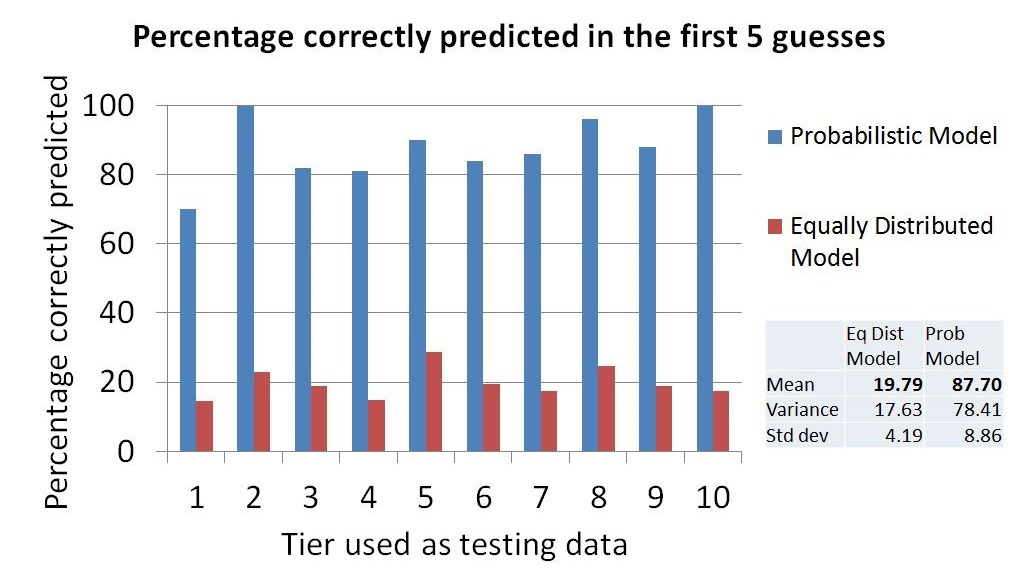
\includegraphics[scale=0.33]{sanity1}
  \caption{ \todo{Additionally I think this graph ight make more
      sense as a table, with variances and averages included.  The legend to the
      side is honestly the important part, and also too small.  Include an
      aggregate/total row.}.   }

\end{figure}

We ran this experiment with all the rows $n$ in the sub-model $TE_{n,m}$ and 
$TP_{n,m}$ for each of the 10 
folds. The results are detailed in Figure~\ref{fig:results10fcv}. As we can see 
in this graph, the red bars represent the results of the percentage of correctly 
predicted instances of the testing data in each particular fold by the top five guesses of the equally distributed approach; while the blue 
bars represent the percentage of correctly predicted instances using the top five 
guesses of the sub-model of each of the folds. We have a mean of 19.79\% 
correctly predicted instances through the different folds when using the equally 
distributed schema, while we get a mean of 87.70\% correctly predicted instances 
through the different folds when using the probabilistic model. 

\subsection{Case study}
\label{sec:casestudy}

\todo{Explanatory note: you have been introducing subsections with temporal
  descriptions: ``after X, we decide to do why.''  Time is not very important in
  papers.  Instead, introduce each subsection with the experimental goal or
  question.  What is the purpose of these experiments?  Avoid phrasing like
  ``the obvious next step'' or ``the natural thing to do'' because they beg the
  question and are weak in terms of motivation.}

We assess the
model's utility in a repair algorithm on a small case study example, constructed
to differ from the code used in the model.  Therefore we evaluated our model
\todo{model, or a repair technique that uses the model?}
with an example of a basic bug in a method as shown in Figure~\ref{fig:initialExample}. The purpose of this method is to calculate the median 
of three numbers, and there is a bug as indicated by the highlighted text where 
instead of $ret = z;$ it should be $ret = x;$ to have a correct output 
for all cases.



\begin{figure}[t]
\begin{lstlisting}[frame=single,style=base]
  public int mid(int x, int y, int z){
    int ret = z;  
    if(y<z){
      if(x<y){
        ret = y;
      }else if(x<z){
        ret = z; @//bug, it should be ret=x;@
      }
    }else{
      if(x>y){
        ret = y;
      }else if(x>z){
        ret = x;
      }
    }
    return ret;
  }	
	\end{lstlisting}
	\caption{Source code of an independent example. Bug to be fixed is annotated and highlighted}
	\label{fig:initialExample}
\end{figure}



%\begin{figure}[!h]
%  \centering
%    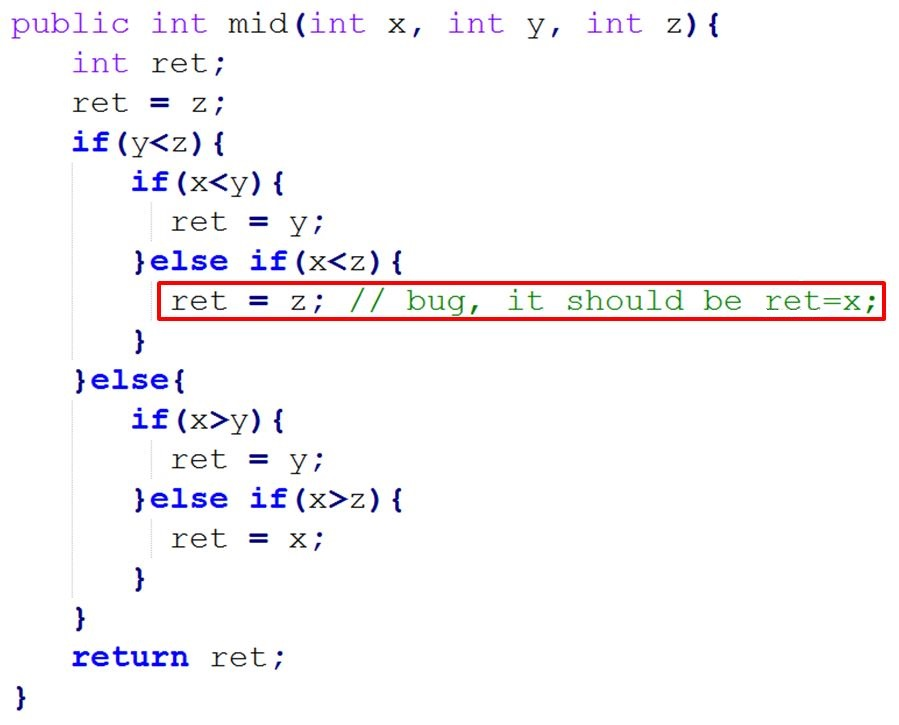
\includegraphics[scale=0.35]{sanity2}
%  \caption{Source code of an independent example. Bug to be fixed is annotated %and highlighted}
%  \label{fig:initialExample}
%\end{figure}

To be able to do this, we forked and extended an open-source Java version of the 
well known\todo{we don't need to call it well known every time it's mentioned,
  it sounds braggy once you know who wrote the paper.  Please remove it here,
  and then this todo.} tool GenProg~\cite{legoues12}.\todo{I might actually cite the TSE
  genprog paper rather than the ICSE 12 paper and also, we should leave the
  footnote out because if anyone goes there and looks at the commit log they
  will see that it's obvious that we did this paper.  That's why I killed the
  footnote that existed previously.} This tool provides the work-flow 
for many generate-and-validate approaches to be implemented. We restructured the 
tool to be able to select the mutation operators between a 
probabilistic model, and the default (equally distributed).

We then ran the tool on the code in Figure~\ref{fig:initialExample} using both 
the probabilistic model and the equally distributed model. Since this is a 
case study for sanity checking, we start by evaluating it on a subset of 
the mutation operators. We first evaluate it in two different sets: 1) Only using the $Replace$ mutation operator, and 2) Using only $Append,~
Remove~and~Replace$ mutation operators. The results are detailed in figures 
\ref{fig:resultsReplace} and \ref{fig:resultsARR}. 

\todo{I can reduce the text here once the other todos in experiments ar addressed}
Generate-and-validate, as explained before, works by creating variants of the 
source code by applying mutation operators to the original source code. 
Therefore, a large number of variants created before finding a patch means that 
it takes longer to find a patch, than a small number of variants. We can imply by this 
that in these graphs, the smaller number of variants in each case, means that 
the patch was found faster, than with a larger number of variants. It is also 
noticeable that this tool uses genetic programming in its workflow, therefore we 
run the tool with 10 different seeds to be able to abstract the results 
and not focus on a particular seed.

In Figure~\ref{fig:resultsReplace} we consider only the mutation operator 
$Replace$, which means that the tool will disregard all other mutation 
operators and will only apply Replace operations using the probabilistic model 
of Replacements. This is because at this step we are evaluating our model in a 
subset of the mutation operators to understand if it makes sense to move forward and 
continue implementing the rest of the mutation operators.

In this graph we can analyze the runs with 10 different seeds, contrasting the 
number of variants it takes to find a patch using the probabilistic approach 
(blue bar), with the number of variants it takes to find a patch using the 
equally distributed approach (green bar). 

As we can derive from the graph, the probabilistic approach was able to find a 
patch faster than the equally distributed for all the seeds tested. In some 
cases as seed 5, 7 and 10, the patch using the probabilistic approach was found 
in one of the first variants, therefore the number is so low that it doesn't 
show in the graph. In average, we found that by using the probabilistic model we 
could find a patch in 23.8 variants, while it took an average of 60.5 variants 
to find a patch using the equally distributed model.

\begin{table}[ht]
\begin{tabular}{lR{0.1cm}R{0.1cm}R{0.1cm}R{0.1cm}R{0.1cm}R{0.1cm}R{0.1cm}R{0.1cm}R{0.1cm}R{0.1cm}R{0.5cm}R{0.5cm}}
\hline
\textbf{Seed} & \textbf{0} & \textbf{1} & \textbf{2} & \textbf{3} & \textbf{4} & \textbf{5} & \textbf{6} & \textbf{7} & \textbf{8} & \textbf{9} & Avrg & StdDev  \\
\hline
\textbf{Prob} & 48 & 19 & 81 & 41 & 0 & 11 & 0 & 25 & 13 & ~~~~0 & 23 & 24 \\

\textbf{Eq Dist} & 49 & 34 & 89 & 98 & 4 & 11 & 80 & 25 & 13 & 202 & 60 & 57\\
\hline
\end{tabular}
\center
  \caption{Number of variants it takes to find a patch (starting at 0) using replace to guide the search for a patch of the case study}
  \label{fig:resultsReplace}
\end{table} 

%\begin{figure}[!h]
%  \centering
%    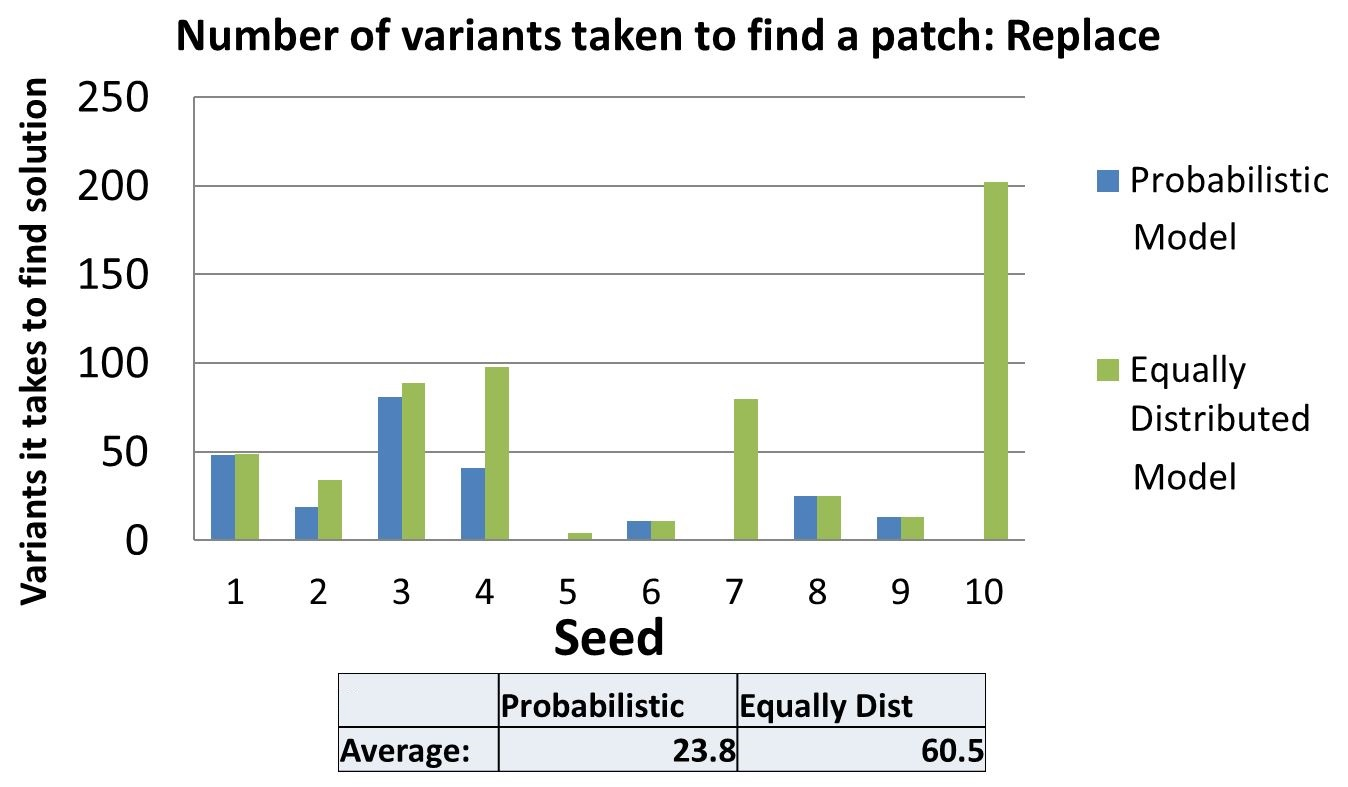
\includegraphics[scale=0.25]{sanity3}
%  \caption{Using replace to guide the search for a patch of the case study}
%  \label{fig:resultsReplace}
%\end{figure}

In Figure~\ref{fig:resultsARR}, we consider three mutation operators: Append, 
Remove and Replace. In this case we can also notice that in seeds 7 and 10 the 
number of variants it takes to find a patch using the probabilistic model is 
close to 1 therefore it is hard to notice it in the graph. In this case the data 
shows that using the probabilistic model we obtain a mean of 22.6 variants 
before finding the patch, while it takes an average of 41.4 variants to find the 
patch using the equally distributed approach. We consider of importance to notice that in both experiments the probabilistic model outperformed the equally distributed model in every single case.

\todo{On all results here: do not separate out by seed.  Report the average and
  standard deviation across successful seeds.  Report random success rate
  (percentage of successful seeds).  You can probably put all that for both
  tables in a single table/figure.  This is because the different seeds are not meaningful.}

\begin{table}[ht]
\begin{tabular}{lR{0.1cm}R{0.1cm}R{0.1cm}R{0.1cm}R{0.1cm}R{0.1cm}R{0.1cm}R{0.1cm}R{0.1cm}R{0.1cm}R{0.5cm}R{0.5cm}}
\hline
\textbf{Seed} & \textbf{0} & \textbf{1} & \textbf{2} & \textbf{3} & \textbf{4} & \textbf{5} & \textbf{6} & \textbf{7} & \textbf{8} & \textbf{9}  & Avrg & StdDev  \\
\hline
\textbf{Prob Model} & 8 & 20 & 23 & 42 & 4 & 11 & 0 & 29 & 80 & ~~~~0 & 22 & 23\\

\textbf{Eq Dist} & 8 & 66 & 23 & 42 & 4 & 11 & 2 & 38 & 81 & 139 & 1704 & 41 \\
\hline
\end{tabular}
\\
\\
%\center
%\begin{tabular}{|lrrr|}
%\hline
%& Average & Variance & Std Dev \\
%\hline
%\textbf{Prob Model} & 22.6 & 563.0 & 23.7\\
%\textbf{Eq Dist} & 41.4 & 1704.0 & 41.3\\
%\hline
%\end{tabular}
%\\
%\center
  \caption{Number of variants it takes to find a patch (starting at 0) using append, remove and replace to guide the search for a patch of 
the case study}
  \label{fig:resultsARR}
\end{table} 
%\begin{figure}[!h]
%  \centering
%    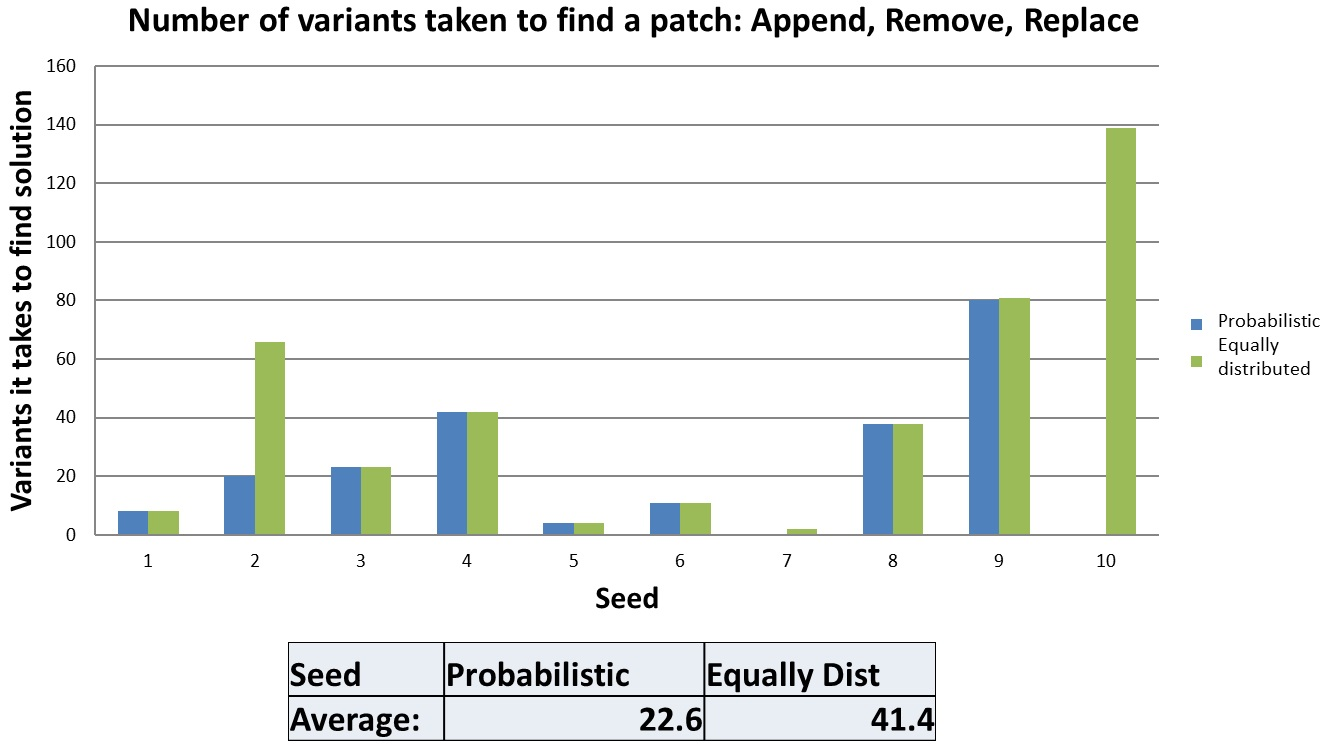
\includegraphics[scale=0.25]{sanity4}
%  \caption{Using append, remove and replace to guide the search for a patch of 
%the case study}
%  \label{fig:resultsARR}
%\end{figure}

\subsection{Single line bug repair}
\label{sec:single}

\todo{See my todo about motivation of subsections at the top of the previous
  subsection and then fix this one.}
After having very successful results in the first two evaluations with a subset of the model, we decided 
to increase our data by building the whole model with 500 projects in Github with more 
stars.\todo{I don't know if this claim is true, if we count considered commits
  rather than projects.  Is it?} This is to generate the largest code base so far to the best 
of our knowledge, surpassing all the previous state of the 
art~\cite{long15,Soto15,zhong15,matias15,xuan16}. 

In our dataset, Template-Based mutations comprise 29.26\% of the corpus; Statement-Edit mutations make up 70.74\% of the 
corpus. Since this idea\todo{...which idea? Also drop the ``seems promising we
  decided...'' and just say what we did.  It's obvious we decided it because we
  did it.} seems promising at this point we decided to implement the rest 
of the mutation operators. We implemented these 16 templates in GenProg4J, and generated the functionality 
to be able to select which subset of mutation operators to apply in a particular 
run.

We evaluate the repair approach on a subset of the Defects4j~\cite{just14}
benchmark.  Defects4j is a database and extensible 
framework providing real bugs to enable reproducible studies in software testing 
research. This database of bugs contains 357 real bugs from 5 
real-world open source programs, and each of these cases is accompanied by a 
comprehensive test suite with test cases that expose the bug. This database also provides 
the corresponding human-generated patch, which is the version of the code written by a human 
developer to patch the bug. Defects4j has previously been 
subject for evaluation of important APR approaches~\cite{Durieux15}.\todo{but we
  don't evaluate on all 357, right?}

We set the size for each population to 40 for consistency with 
previous work~\cite{legoues12,kim2013}\todo{does Par say the population size
  they use? Also add generation count, or say we used rsrepair instead of
  genprog as a search strategy (if that's true).  Say how many seeds we ran per.}  and a timeout of 4 hours since there is 
the need of several generations of mutant creations needed to assess the 
performance of this approach~\cite{arcuri11}.

For this evaluation we tested the mutation operators using three different sets 
of operations: 1) Statement-Edit mutations only 2) Template-based mutations 
only 3) All mutations.  \todo{why?}
Since historically automatic program repair has worked better with single line 
patches, we decided to first test bugs that required a single line edit to get 
patched. We analyzed the first 3 bugs from each of the projects that required a 
single line edit.\todo{move the footnote content so that it's not a footnote.} \footnote{The bugs that met this criteria are the following: Chart 1, 
Chart 8, Chart 20, Closure 10, Closure 14, Closure 18, Lang 6, Lang 16, Lang 21, 
Math 2, Math 5, Math 10, Time 4, Time 16 and Time 19.}

Several evaluations in the past use an off-the-shelf fault localization
technique when evaluating a new way to navigate the search space, which
introduces a lot of noise and randomness to the result of the patch creation and
selection process. To diminish the degree of randomness in this experiment, we
will be using Human Injected Fault Localization, a technique\todo{It's not ``A
  technique'' like a previously-proposed approach.  We're
  overstating what we did and it sounds like we're bullshitting.  Just say: ``to
  control for randomness and inefficiency and isolate the effect, we manually
  identify faulty locations to be repaired to isolate the effect of X.''  Other
  work has in fact done this (...Par, one of the experiments in the ICSE 2012
  paper), and you might find a delicate way to say that.}. in which the
researcher indicates to the APR approach the section of the code that contains
the defect. In these cases we picked the faulty statements to be the statements
which the human developers modified to patch the code. 

From these 15 bugs we were able to find patches for 5 of them as described in
Table~\ref{tab:singleLineBugs}. Results show the average of results on 
20 different seeds.  

In the first row of Table~\ref{tab:singleLineBugs} (Closure \#10) we can see
that in all three comparisons (Statement-Edit Only, Template-Based Only, and All
mutations), the approach using the probabilisitc model performs better than its
counterpart using the equally distributed model. This happens as well in all
cases of bugs Math \#2 and Time \#19 except for the cases where no patch was
found. By contrast \todo{Your original phrasing was ``different from this'',
  which isn't grammatical.  I
  mention it just because it's a phrase you've used elsewhere and I keep
  rephrasing but if I don't tell you, you won't learn. ;-)}, for bugs Chart \#1 and Closure \#18 the equally
distributed approach finds a patch faster in average. This is due to the fact
that removal mutations such as Deletion and Expression Changer are more likely
to be picked by the equally distributed model than the probabilistic model since
developers use these editions less often than others. But these editions have
been seen in the past to make the test cases pass even if the edition did not
fixed the bug as per the opinion of developers as indicated in~\cite{kim2013}. 

Our results also show that applying mutation operators from both categories
together, benefits the process by finding the patch faster, than when
restricting the mutation operator pool to just one of the categories. For the
Statement-Edit category: 3 out of 6 were fixed faster when combining it with
Template-Based mutations, and 3 out of 6 were slower. For the Template-Based
category: 4 out of 8 were fixed faster when combining it with Statemtent-Edit
mutations, 2 out of 8 were the same, and 2 out of 8 were slower. 

\begin{table*}\centering
\ra{1.3}
	\resizebox{\textwidth}{!}{
\begin{tabular}{|r|rr|rr|rr|rr|rr|rr|}
\hline
  &\multicolumn{4}{c|}{\textbf{Stmt-Edition}} & \multicolumn{4}{c|}{\textbf{Temp-Based}} & \multicolumn{4}{c|}{\textbf{All mutations}} \\  
 \hline
 \textbf{Bug Name}  & \multicolumn{2}{c|}{\textbf{Equally Dist}} & \multicolumn{2}{c|}{\textbf{Probabilistic}} & \multicolumn{2}{c|}{\textbf{Equally Dist}} & \multicolumn{2}{c|}{\textbf{Probabilistic}} & \multicolumn{2}{c|}{\textbf{Equally Dist}} & 
\multicolumn{2}{c|}{\textbf{Probabilistic}} \\

 Closure \#10 & \color{OliveGreen}{221.0}& \color{blue}{100\%} & \color{OliveGreen}{179.5} &\color{blue}{100\%} & \color{OliveGreen}{175.1}&\color{blue}{100\%} & \color{OliveGreen}{121.3}&\color{blue}{100\%} & \color{OliveGreen}{163.3}&\color{blue}{100\%} & \color{OliveGreen}{157.4}&\color{blue}{100\%} \\

 Closure \#18 & \multicolumn{2}{c|}{Not found} & \multicolumn{2}{c|}{Not found} & \color{OliveGreen}{36.2}&\color{blue}{100\%} & \color{OliveGreen}{197.5}&\color{blue}{100\%} & \color{OliveGreen}{45.0}&\color{blue}{100\%} & \color{OliveGreen}{139.0}&\color{blue}{100\%} \\

 Math \#2 & \multicolumn{2}{c|}{Not found} & \multicolumn{2}{c|}{Not found} & \color{OliveGreen}{109.4}&\color{blue}{0\%} & \color{OliveGreen}{39.6}&\color{blue}{0\%} & \color{OliveGreen}{109.4}&\color{blue}{0\%} & \color{OliveGreen}{39.6}&\color{blue}{0\%} \\

 Time \#19 & \color{OliveGreen}{94.1}&\color{blue}{100\%} & \color{OliveGreen}{80.7}&\color{blue}{100\%} & \multicolumn{2}{c|}{Not found} & \multicolumn{2}{c|}{Not found} & \color{OliveGreen}{135.1}&\color{blue}{100\%} & \color{OliveGreen}{91.9}&\color{blue}{100\%} \\

 Chart \#1 & \color{OliveGreen}{1.8}&\color{blue}{0\%} & \color{OliveGreen}{7.3}&\color{blue}{0\%} & \color{OliveGreen}{4.9}&\color{blue}{0\%} & \color{OliveGreen}{19.0}&\color{blue}{0\%} & \color{OliveGreen}{2.2}&\color{blue}{0\%} & \color{OliveGreen}{4.8}&\color{blue}{0\%} \\

\hline
 
\end{tabular}
}
\ra{1.3}
		\caption{Value on the left of each slot (green): Number of variants taken to find a patch in single line bugs. Value on the right of each slot (blue): Percentage according to the number of patches that passed the second test suite}\label{tab:singleLineBugs}
\end{table*}


\paragraph{Quality assessment:}\todo{This comes a little bit out of nowhere; it
  may be worth alluding to it at least at the top of the subsection and even in
  the contributions list.  ALso in motivating the held-out test suite approach
  for assessing you should cite Smith15, and maybe even the TSE 12 GenProg
  paper, which used held out workloads on case study patches}
To assess the quality of the patches generated by both models we need an
independent validation mechanism. In this study we automatically build a second
test suite of test cases that describes the same behavior as the test suite that
guides the search process. This second test suite will be composed by a
different set of test cases, so we can test the same behavior but so that we can
also generalize the patch to different descriptions of the same behavior and not
to overfit to a particular set of test cases taken to guide the search. To
achieve this, we used the popular automatic test suite generation tool for Java,
Randoop~\cite{pacheco07}. 

For each of the bugs that we were able to create a patch for, we have
subtracted\todo{...subtracted?  I'm not sure what you mean.}
the source code of the human patch provided by Defects4j to take this as a
description of the behavior of the program after the bug has been fixed, and we
have run Randoop for ten minutes (six times the default value, to make sure we
have enough test cases to test the validity of the patch) on this version of the
code to get a different test suite\footnote{Available at: https://goo.gl/YbFeql}
than the one used to guide the search.  

We then ran this second test suite on the patch generated by both models and we
obtained the results noted in Table~\ref{tab:singleLineBugs}. We noticed a
constant behavior regarding the different sets of mutations. In this sample, if
a model is able to find a patch faster, then that also happens independent of
the mutation set used. We notice that in the majority of cases when the
probabilistic model was used, we were able to find a patch faster that when
using the equally distributed approach. In this evaluation, we also notice that
the quality of patches produced is constant; either the tool produces patches in
the different seed that all pass the second test suite, or it produces patches
that none of them pass the second test suite.  

%\subsection{Bugs fixed with a multi line edit within a function}
%Last evaluation with the bugs we found had a fix

\subsection{Association Rule Mining} \label{armRes}
\todo{See my notes on ARM in approach about the content that needs to move
  there.  Then I'll reread.}

\textbf{Mutation operator and replacement rules:}
To create these association rules among several mutation operators, we mine the
transactions made out of the commits created by humans in the corpus of projects
studied and we look for rules that have at least 90\% Confidence, where
Confidence is an indication of how often the rule has been found to be true.  
These rules are ranked by their confidence; in this case, the top 5 rules shown
below have a confidence of a 100\% which means that in 100\% of the cases
studied, every transaction that showed the antecedent also shows the consequent;
and they are obtained with a 1\% support, which means that each of these rules
individually show in at least a 1\% of all the transactions of the overall
corpus. We show the 5  top association rules found for the mining of single edit
mutation operators. 


%Minimum support: 0 (1 instances)
%Minimum metric <confidence>: 0.9
%Number of cycles performed: 20
\begin{itemize}
\item Replace \& Delete $\implies$ Append
\item Delete \& AddNullCheck $\implies$ Append
\item Replace \& SeqExchanger $\implies$ Append
\item Replace \& ParamReplacer $\implies$ Append
\item Delete \& CasteeMutator $\implies$ Append
%\item Replace \& Delete \& ParamReplacer $\implies$ Append
%\item Replace \& AddNullCheck $\implies$ Append
%\item Replace \& Delete \& SeqExchanger $\implies$ Append
%\item Delete \& ExpressionAdder $\implies$ Append
%\item Delete \& AddNullCheck \& ParamReplacer $\implies$ Append
\end{itemize}

Append is the most common single edit mutation operator. This behavior is
reflected in the fact that it is the most common consequent being the consequent
in 5 out of 5 of the top 5 association rules. The authors are showing the top 5
association rules to give an example of what the rules look like. If the reader
would like to know the full list of association rules mined in this study, the
authors have made available the full list with over 12.000 rules with over 90\%
Confidence and 0.01\% Support.\footnote{https://goo.gl/UT8QbI} 
%REPLACE FOR CAMERA READY: https://github.com/mausotog/ReplacementsEmpiricalStudy/blob/master/ResultsAssociationRuleMiningMutOperators.txt

Similar to the case detailed before, we have analyzed the association rules for the replacements model. We obtained the following rules with a 0.01\% Support and 90\% Confidence.
10 Best rules found:
%Minimum support: 0.0001 (1 instances)
%Minimum metric <confidence>: 0.9
%Number of cycles performed: 20
\begin{itemize}
\item Block replaces ReturnStatement \& ExpressionStatement replaces IfStatement $\implies$ Block replaces IfStatement
\item VariableDeclarationStatement replaces AssertStatement $\implies$ SwitchCase replaces BreakStatement
\item EnhancedForStatement replaces TryStatement $\implies$ ExpressionStatement replaces ReturnStatement
\item ForStatement replaces TryStatement $\implies$ ExpressionStatement replaces VariableDeclarationStatement
\item VariableDeclarationStatement replaces EnhancedForStatement $\implies$ ExpressionStatement replaces VariableDeclarationStatement
\item VariableDeclarationStatement replaces ForStatement $\implies$ ExpressionStatement replaces VariableDeclarationStatement
\item ForStatement replaces TryStatement $\implies$ IfStatement replaces TryStatement
\item VariableDeclarationStatement replaces ForStatement $\implies$ ForStatement replaces TryStatement
\item ForStatement replaces TryStatement $\implies$ VariableDeclarationStatement replaces ForStatement
\item VariableDeclarationStatement replaces ForStatement $\implies$ IfStatement replaces TryStatement
\end{itemize}

Similar to the one described above, the authors have made available the full list of association rules with over 90\% Confidence and 0.01\% Support.\footnote{https://goo.gl/omk60t}
%REPLACE FOR CAMERA READY: https://github.com/mausotog/ReplacementsEmpiricalStudy/blob/master/ResultsAssociationRuleMiningReplacements.txt

\subsection{Discussion} \label{discussion}

In this paper we are tackling specific 
challenges regarding the way in which mutation operators are chosen, we provide 
a probabilistic model that describes the way in which humans give preference to 
some mutation operators over others, and have analyzed how these single edit 
source code changes can be chained together to form multi edit changes.

To do this we have analyzed the way in which humans create single edit 
source code changes and we have created a set of association rules that describe 
how often different sets of mutation operators can predict the change that will 
come next and how often subsets of mutation operators are applied together.

There is a tension between the Support and the Confidence in the transaction 
base, in particular the transaction base considered in this study, in which we 
evaluate the different mutation operators being applied to source code in bug 
fixing commits. 

If we increase the Confidence and decrease the Support we will obtain rules in 
which the priority is that every time that the antecedent happens, the 
consequent will happen as well. With this approach we may obtain rules that 
don't happen very often, but every time that they happen in the analyzed corpus, 
there is a high confidence that the rule will be correct. On the other hand, if 
we increase the Support and decrease the Confidence we would obtain rules that 
are guaranteed to happen in a certain percent of the corpus, which means, that 
the relationship described by the rules, happen often, but confidence is 
sacrificed, which means that there will be a higher percentage of the 
transactions in which the antecedent is present, but the consequent is not. 

Regarding Table~\ref{tab:singleLineBugs}, there are two of these bugs in which
the equally distributed model performed better than the probabilistic
model. This is due to the fact, that the mutations needed to be applied in the
source code for it to pass all the test cases, are mutation operators that are
not usually applied by humans, and therefore they have a smaller probability of
being chosen by the probabilistic model, and this is exposed as a larger number
of variants needed to find these unusual mutation operators. 

We also notice that applying different probabilities when constructing variants
does not make the patches found in either of the models more likely to pass a
second test suite for these five bugs. Further evaluation should be performed to
determine if one of the models creates higher quality patches than the other. 
  
\subsection{Threats to Validity} \label{threatsVal}

\paragraph{Internal validity:}
Regarding possible errors in our implementation and experiments, to run our comparison with Genprog, we used Genprog4Java\footnote{https://bitbucket.org/clegoues/genprog4java/}, a publicly available version of Genprog created by the original creators of Genprog. Unlike other similar versions who have tried to replicate Genprog in a Java context, this version is written by the creators of Genprog who understand and know all the details of the original implementation, therefore mitigating the possibility of errors in the translation process. Regarding the PAR templates, we have had to write the templates ourselves due to the fact that the implementation of the PAR templates has not been made publicly available by the authors of that approach. In order to mitigate this, we made our implementation of the templates publicly available 
%REMOVE THIS FOR CAMERA READY
%in the project mentioned before 
to be checked and used in the future by ongoing researchers.

\textbf{External validity:} 
Regarding the generalizability of our findings, the authors acknowledge the concern that this idea might not generalize to external datasets and further real life bugs. To attenuate this concern, the authors have evaluated their experiment on a state of the art bug-mining platform which consists of five different real life well known open source projects. We analyzed 15 different real life bugs from different projects in very different areas of knowledge (eg, math, language, technology, time representation, graphical interphase). 

\textbf{Construct validity:}
Regarding the suitability of our evaluation metrics, the authors evaluate patch quality by running the generated patches through a second test suite created from a human patch, which is to a certain extent a biased measure since we can't guarantee that the human created patch is perfect. Nevertheless, this is a best known practice, especially when compared to the the approach used previously in similar experiments in which a biased human developer would judge whether he/she considered the patch was correct or not.

\section{Related Work} \label{relatedWork}

There have been previous efforts to create a model based on human behavior by Soto et al~\cite{Soto15} 
where the researchers built a probabilistic model of the replace mutation 
operator only, based in 
an instance count of each statement type using the platform 
BOA,~\cite{dyer2013} and making an initial model of the replacement mutation 
operator only. HDRepair~\cite{xuan16} has also tried to tackle this problem by 
creating a repair approach that uses a modified stochastic search
technique in which the researchers use fix history
to help assess their fitness. The fitness of the generated
fix candidates is determined by the frequency with which the changes included in a given patch occur in the corpus using a Graph-based representation of the bug fixes.

Prophet~\cite{long15} is also an approach that has done previous work in this 
area, where the researchers built a 
probabilistic model for a subset of the mutation operators (the SPR transformation schemas), with a training set 
of 8 different projects. They then rank the candidate patches according to this model and evaluate them in that order. Our approach follows this intuition to mimic human behavior; we apply this knowledge when creating the patch candidates, as opposed to Prophet, which applies this knowledge afterwards. 

A similar case is studied in ``An empirical study on 
real bug fixes"~\cite{zhong15} with a smaller number of projects (6) and a 
smaller set of 
mutation operators (3), and also by Matias\todo{This is his first name.
  Martinez is his last name.  Please cite appropriately} and Monperrus~\cite{matias15} with 14 
projects. To the best of our knowledge a full set of mutation 
operators hasn't been studied and compared in the past, as neither has a study 
consider such a vast diversity of projects to build a probabilistic model. In 
order to counter the 
risk of overfitting to a small set of training projects as performed before, our 
current study trains the model with 500 projects, which covers a vast diversity 
of dominions and bug fixing styles.

\todo{I strongly believe there's more work here.  What is cited by Martinez and
  Monperrus and by Zhong and Su?  Other work in mining for human bug fixing
  behavior is appropriate as well.}

\section{Conclusion} \label{conclusion}

In this study we analyze the way in which current state of the art automatic 
program repair approaches select mutation operators to create candidate 
patches. We analyze, categorize and compare the mutation operators being used by 
state of the art approaches. We analyzed the last 100 bug fixing commits from the
500 projects in Github with most stars, which is the largest corpus analyzed to date
to the best of our knowledge, and we created a two level probabilistic model regarding 
the likelihood of mutation operators to be selected as humans select them.

We evaluated our approach in three different ways: by performing 10 fold cross 
validation of the model, by comparing the equally distributed model with the probabilistic model by running an initial independent example; and finally by  comparing the two models by running them on 15 bugs using the database of bugs and extensible 
framework Defects4j. For these bugs, we measured the number of variants it takes to find the patch and the quality of patches by using a second automatically created test suite using Randoop. 

According to the 10 fold cross validation\todo{please rephrase, because as we've
  discussed to death, the cross validation is not the thing doing the assessment.}, the probabilistic model outperforms
the equally distributed model by a factor of 4 when looking at the first five
guesses of each model. When running an initial independent example, the
probabilistic model outperformed the equally distributed model by a factor of 3
and a factor of 2 accordingly. And when running in the bugs obtained by
Defects4j, the probabilistic model outperformed the equally distributed model in
the majority of the cases. We did not find a difference in the quality of
patches produced by each of the approaches in this sample. 

Finally, we have analyzed a field that has been understudied in the past and which covers 
the vast majority of bug fixes in software systems, which is Multi-edit source code changes. 
We have created a set of association rules using Apriori, a state of the art
methodology for association rule mining based on the analyzed corpus. The authors have
made an initial analysis of how single-edit source code changes can be chained together 
to become multi-edit source code changes the way humans do it.



% conference papers do not normally have an appendix


% use section* for acknowledgment
\section*{Acknowledgments}
The acknowledgments section will be added for the camera ready version. 





% trigger a \newpage just before the given reference
% number - used to balance the columns on the last page
% adjust value as needed - may need to be readjusted if
% the document is modified later
%\IEEEtriggeratref{8}
% The "triggered" command can be changed if desired:
%\IEEEtriggercmd{\enlargethispage{-5in}}

% references section

% can use a bibliography generated by BibTeX as a .bbl file
% BibTeX documentation can be easily obtained at:
% http://mirror.ctan.org/biblio/bibtex/contrib/doc/
% The IEEEtran BibTeX style support page is at:
% http://www.michaelshell.org/tex/ieeetran/bibtex/
%\bibliographystyle{IEEEtran}
% argument is your BibTeX string definitions and bibliography database(s)
%\bibliography{IEEEabrv,../bib/paper}
%
% <OR> manually copy in the resultant .bbl file
% set second argument of \begin to the number of references
% (used to reserve space for the reference number labels box)
%\begin{thebibliography}{1}

%\bibitem{IEEEhowto:kopka}

%\end{thebibliography}

\bibliographystyle{abbrv}
\bibliography{sigproc}  % sigproc.bib is the name of the Bibliography in this case
% You must have a proper ".bib" file
%  and remember to run:
% latex bibtex latex latex
% to resolve all references



% that's all folks
\end{document}


